\documentclass[fleqn,usenatbib]{mnras}
\usepackage[T1]{fontenc}
\usepackage{ae,aecompl}
\usepackage{graphicx}
\usepackage{amsmath,amssymb}
\usepackage{bm}
\usepackage{booktabs}
\usepackage{xcolor}
\usepackage{tikz}
\usetikzlibrary{arrows.meta,positioning,fit,calc}
\hypersetup{hypertexnames=false,colorlinks=true,linkcolor=blue!50!black,citecolor=blue!50!black,urlcolor=blue!50!black}

\newcommand{\todo}[1]{}
\newcommand{\asz}{A_\mathrm{SZ}}
\newcommand{\alsz}{\alpha_\mathrm{SZ}}
\newcommand{\ssz}{\sigma_\mathrm{SZ}}
\newcommand{\blens}{\beta_\mathrm{lens}}
\newcommand{\slens}{\sigma_\mathrm{lens}}
\newcommand{\qobs}{q_\mathrm{obs}}
\newcommand{\qtrue}{q_\mathrm{true}}
\newcommand{\msun}{\mathrm{M}_\odot}
\newcommand{\sfinder}{\sigma_\mathrm{finder}}
\newcommand{\classyszlite}{\textsc{classy\_szlite}}
\newcommand{\omc}{\omega_\mathrm{c}}
\newcommand{\omb}{\omega_\mathrm{b}}
\newcommand{\Omm}{\Omega_\mathrm{m}}
\newcommand{\cov}{\mathcal{C}}

\title[Cluster counts from maps]{Cluster counts from maps: simulation-based inference of
Sunyaev--Zel'dovich cluster abundances with a map-level forward model}
\author[]{}
\date{}
\pubyear{2026}

\begin{document}
\label{firstpage}
\pagerange{\pageref{firstpage}--\pageref{lastpage}}
\maketitle

\begin{abstract}
We present simulation-based inference of thermal Sunyaev--Zel'dovich (tSZ) cluster counts in which every
training simulation runs the cluster finder on simulated multi-frequency maps, to our knowledge the first
of its kind. Our simulator paints haloes into six Simons Observatory (SO) frequency maps with the cosmic
microwave background (CMB) and goal-depth noise, and runs a matched-filter finder. On one GPU, a survey of
40.7 per cent of the sky takes 1.6\,s and a training set of 10\,000 surveys 4.6\,h. At this sky fraction, the
posterior is within 0.11 widths (posterior standard deviations) of the truth, and its 90 per cent
intervals contain the truth for 0.88--0.91 of 500 prior skies. On the same skies, we compare it with
catalogue models calibrated on map-level mocks, which have to carry the finder's confusion noise (4--8 per
cent), search over positions and sizes, neighbours and upward error tail. A model calibrated at the
true parameters is within 0.2 widths at that point in $\sigma_8$, the cold dark matter density and the
tSZ--mass log-amplitude, but too narrow or off-centre across the prior. Calibrated at 25 points across
the prior, it has close to correct coverage for these three but leaves the slope of the relation
0.6--0.7 widths high, which we attribute to the tail. As a reference, the uncalibrated model, with a noise
table for the instrument and the CMB only, is biased by up to 8.3 widths on our skies, showing the size of
the finder's effects at goal depth.
\end{abstract}


\begin{keywords}
galaxies: clusters: general -- cosmological parameters -- methods: statistical -- cosmic background radiation
\end{keywords}

\section{Introduction}\label{sec:intro}

The abundance of galaxy clusters as a function of mass and redshift traces the growth of structure, since
it depends, through the halo mass function \citep[e.g.][]{Tinker2008}, on the amplitude of matter
fluctuations, $\sigma_8$, and on the matter density, $\Omm$. Clusters can be detected through the thermal
Sunyaev--Zel'dovich (tSZ) effect \citep{SZ1972}, in which the hot gas of a cluster scatters the photons of
the cosmic microwave background (CMB), leaving a decrement at low frequencies and an excess at high
frequencies. Because the tSZ surface brightness does not fall with redshift, a tSZ survey detects massive
clusters out to high redshift \citep{Carlstrom2002}. The Simons Observatory \citep[SO;][]{SO2019} will map
a large fraction of the sky in six frequency channels with arcminute resolution and low noise. It will therefore detect many more clusters than current surveys and measure their masses with CMB lensing
\citep{MelinBartlett2015,Madhavacheril2017}.

Planck \citep{Planck2016XXVII,Planck2016XXIV}, the South Pole Telescope \citep[SPT;][]{Bocquet2019,
Bocquet2024} and the Atacama Cosmology Telescope \citep[ACT;][]{Hasselfield2013,Hilton2021} have built tSZ
cluster catalogues and used them for cosmology. All of them find clusters mainly with multi-frequency
matched filters \citep{Herranz2002,Melin2006} (Planck also with PowellSnakes). A matched filter combines
the frequency maps with the known tSZ spectrum and a template of the cluster profile, and returns a
signal-to-noise $q$ at each position and template size. The cosmological analyses of these catalogues work at the catalogue
level, building the likelihood of the observed counts from the mass function, a relation between the tSZ
signal and mass, and a model of how the finder measures each cluster. In this model, the mean
signal-to-noise of a cluster is its tSZ signal divided by the noise of the filter, and its measured $q$
scatters around that mean with unit Gaussian scatter. Analyses of data usually measure the filter noise
on the observed maps, whereas forecasts take it from a noise table computed for the instrument and the
CMB. In addition, SPT accounts for the rise in measured significance caused by the search over positions
and sizes, with $\langle q\rangle=\sqrt{\bar q^2+3}$ for a cluster of unbiased significance $\bar q$
\citep{Vanderlinde2010}. Likelihoods of this kind are implemented in the \textsc{cosmocnc} package
\citep{ZubeldiaBolliet2024}.

In simulation-based inference (SBI), the likelihood is replaced by simulations \citep{Cranmer2020}, and a
neural network trained on pairs of parameters and simulated data returns the posterior directly
\citep{Papamakarios2016,Alsing2019}. For cluster counts, SBI thus removes the need to write in closed form
the likelihood of binned or unbinned counts, of their scatter and of their selection. \citet{Zubeldia2025}
applied it to an SO-like survey with a CMB-lensing mass observable. Their simulator draws haloes from the
mass function, assigns each halo a tSZ signal and a lensing signal-to-noise, and applies a catalogue-level
model of the finder with a noise table for the instrument and the CMB. It then compresses each catalogue
into 21 numbers, namely the counts in bins of $q$ and redshift and the mean lensing signal-to-noise of the
detections. Similarly, \citet{Regamey2026} applied SBI to mock X-ray cluster surveys, with a forward model
of the selection. In both cases, however, the simulations are of the catalogue, not of the maps. Since a
neural posterior converges to the posterior of the model that generated its training simulations, it can
be no more correct than that model. It can also be overconfident when the network is not well trained
\citep{Hermans2022}, and coverage tests are therefore needed.

A catalogue model therefore has to carry the finder's behaviour on the maps, and calibrating it on the
maps is standard practice. Written with a noise table for the instrument and the CMB, as in forecasts,
the model leaves out three effects of the finder: confusion noise, the search lift and neighbours; and it
assumes Gaussian scatter, which the finder's errors break through an upward tail. Confusion noise arises
because the maps also contain the tSZ signal of every other halo, most of them too faint to detect, and the
finder measures its noise from those maps. The search lift arises because the model takes the position
and size of each cluster as known, whereas the finder searches over positions and sizes and keeps the
maximum of $q$, which raises the $q$ of faint clusters. \citet{Vanderlinde2010} describe this lift with
a fixed correction. Neighbours, finally, are nearby clusters that add their signal to
each other's peaks on the maps and can be merged into one detection. The selection of a tSZ survey is
known to depend on the size of a cluster and not only on its flux \citep{Melin2005}. Current analyses include this dependence through the cluster size in the noise table. The effects above, however, also
depend on the total tSZ signal on the sky, and hence on the cosmological and scaling-relation parameters
that the analysis infers. A noise measured on the data maps includes the confusion noise of the observed
sky, but not the search lift, the change of the scatter with the parameters or the upward tail. Moreover,
in SBI every simulated sky has its own noise, so that the simulator has to produce it, or a calibration
has to follow it through the parameters.

A map-level simulator avoids these assumptions, since it paints the haloes into frequency maps, adds the
CMB and the noise, and runs the finder on the maps as on the data. Its output can then be compressed into
the same summary as the catalogue and used to train a neural posterior. Map-level SBI has been applied to
weak-lensing maps \citep{Jeffrey2021} and, recently, to the tSZ field itself \citep{EmbilVillagra2026},
which also carries information through its power spectrum \citep{Bolliet2018,Planck2016XXII} and its
one-point distribution \citep{Hill2014}. Here we keep the cluster counts as the data and ask two
questions: whether SBI can use a forward model that runs the finder on the maps at the scale of an SO
survey, and how such an inference compares with catalogue models calibrated on the maps. Map-level
simulations are expensive, however, and SBI needs many of them. To our knowledge, no inference of cluster
counts has yet run the finder on simulated multi-frequency maps in every training simulation. To make this
affordable, we have implemented the simulator and the finder in \classyszlite{}, a JAX
\citep{Bradbury2018} package from the \textsc{class\_sz} project \citep{Bolliet2023}. On one GPU, a
survey of 10 per cent of the sky is then simulated in 0.42\,s and a survey of 40.7 per cent in 1.6\,s.

In this paper, we train neural posteriors on map-level simulations of an SO-like survey with the
goal-depth forecast noise of \citet{SO2019}, the deepest of its noise levels. We then compare them, on the same simulated skies, with posteriors trained on
catalogue models. We adopt the summary and the form of
the catalogue model of \citet{Zubeldia2025}, as well as their prior with narrower flat ranges, under which
the slope $\alsz$ of the tSZ--mass relation has a flat prior (Section~\ref{sec:sims:survey}). We express
biases in units of the posterior standard deviation, which we call the posterior width. We find that the
map-level posterior is within 0.11 widths of the truth at 40.7 per cent of the sky and within 0.12 widths
at 10 per cent. It also has close to correct coverage across the prior, since its 90 per cent intervals
contain the truth for 0.88--0.91 of 500 prior skies at 40.7 per cent of the sky. At 10 per cent the range
is 0.86--0.90, and only its $\alsz$ intervals are slightly too narrow. At each
survey size, the map-level posterior combines five networks trained with different seeds, and the results
are robust to the seed (Appendix~\ref{app:robust}). At 40.7 per cent of the sky, a training set of
10\,000 surveys takes 4.6\,h on one GPU, and the whole comparison about 6 GPU hours and 4 CPU hours.

We then calibrate the catalogue model on map-level simulations, both at one point and across the prior,
so that it carries the effects described above. Of these, the confusion noise, which is the tSZ signal of
faint haloes, raises the finder's noise by 4--8 per cent, and the search lift changes with the parameters.
Neighbours widen the scatter and can capture the detection of a cluster, so that the cluster is not
matched. In addition, the calibration has to carry the upward tail. The one-point calibration uses the
finder's noise measured on map-level mocks at the true parameters. At those parameters it is within 0.2
widths of the truth in $\sigma_8$, the cold dark matter density $\omc$ and the log-amplitude $\asz$ of the relation, and it leaves $\alsz$ 0.5
widths high. Across the prior, however, its intervals are too narrow or
off-centre. The noise-level calibration, which follows the parameters through
the finder's noise level, has close to correct coverage for $\sigma_8$, $\omc$ and $\asz$. However, it leaves $\alsz$ 0.6--0.7 widths high with intervals that are too narrow, which we attribute to the upward tail.

Finally, as a reference, we run the uncalibrated catalogue model, that is, the form of
\citet{Zubeldia2025} with a noise table for the instrument and the CMB only, as used in forecasts
(Section~\ref{sec:sims:catalogue}). On our map-level skies, this model is biased by up to 8.3 widths at
40.7 per cent of the sky and by 5.3 widths at 10 per cent, mostly in $\sigma_8$ and $\alsz$. This bias
shows the size of the finder's effects at goal depth with a flat prior on $\alsz$. For the reasons given
in Section~\ref{sec:discussion:scope}, we expect it to be smaller at higher noise, with a noise measured on
the maps or with informative priors on the relation.

The paper is organised as follows. In Section~\ref{sec:sims} we describe the two forward models, namely
the map-level simulator with its finder and the catalogue-level model, and in
Section~\ref{sec:inference} the neural posterior estimation and the checks of bias and coverage. We
compare the finder with the catalogue model, halo by halo and in the counts, in Section~\ref{sec:finder}. In Section~\ref{sec:calibration} we build calibrated catalogue models from
map-level simulations and describe the upward tail that they miss. We then compare the posteriors in
Section~\ref{sec:results}, starting with the map-level posterior and followed by the calibrated models and
the uncalibrated reference. In Section~\ref{sec:discussion} we discuss map-level inference at survey
scale, where the calibrated models fall short, the scope of the uncalibrated reference and the limitations
of the simulator, before concluding in Section~\ref{sec:conclusions}. Finally, we check the robustness of
the neural posteriors in Appendix~\ref{app:robust}.

% =====================================================================
\section{Simulations}\label{sec:sims}
% =====================================================================

In this section we describe the two forward models of the same survey that we compare. Both start from the same parameters and the same haloes and end in the same 21 numbers. As in
\citet{Zubeldia2025}, these are the cluster counts in bins of signal-to-noise and redshift and the mean
CMB-lensing signal-to-noise of the detected clusters. They differ in how a halo becomes a detection
(Fig.~\ref{fig:pipeline}). The map-level simulator paints every halo into six frequency maps, adds the
lensed CMB and the instrument noise, and runs a cluster finder on the maps. In contrast, the
catalogue-level model replaces the maps and the finder by a noise table and a Gaussian scatter. In
Section~\ref{sec:calibration} we then calibrate the catalogue path on map-level mocks, replacing the noise
table by the finder's noise and the unit scatter by equation~(\ref{eq:qobs_fit}).

\begin{figure*}
\centering
% Pipeline diagram: map-level path (top), catalogue path (bottom; the
% uncalibrated catalogue model), and what
% the catalogue path leaves out (middle). Only the tikzpicture; wrap it in a
% figure* in the text. Fits the two-column text width (about 17 cm).
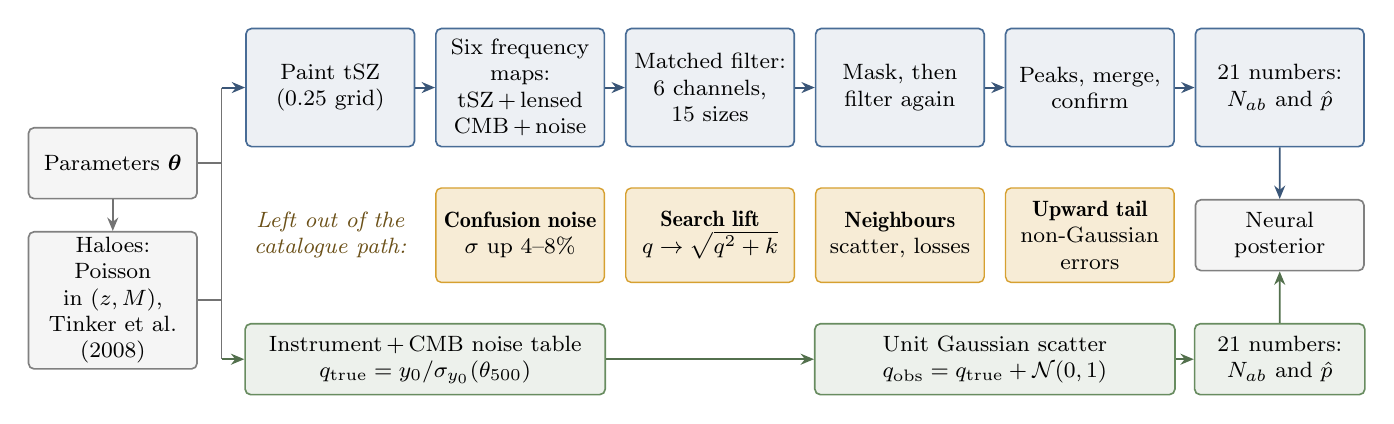
\begin{tikzpicture}[
    font=\footnotesize,
    >={Stealth[length=1.7mm,width=1.4mm]},
    box/.style={draw, rounded corners=2pt, align=flush center, line width=0.6pt,
                inner sep=2pt},
    mapbox/.style={box, draw=mapcol, fill=mapcol!10, text width=20mm,
                   minimum height=15mm},
    catbox/.style={box, draw=catcol, fill=catcol!12, minimum height=9mm},
    inbox/.style={box, draw=black!50, fill=black!4, text width=20mm},
    note/.style={draw=notecol, fill=notecol!20, rounded corners=2pt,
                 align=flush center, inner sep=2pt, line width=0.5pt,
                 text width=20mm, minimum height=12mm},
    maparr/.style={->, draw=mapcol!80!black, line width=0.7pt},
    catarr/.style={->, draw=catcol!80!black, line width=0.7pt},
    inarr/.style={draw=black!55, line width=0.7pt},
  ]
  \definecolor{mapcol}{RGB}{72,108,150}
  \definecolor{catcol}{RGB}{104,140,96}
  \definecolor{notecol}{RGB}{214,160,48}

  % ---- inputs --------------------------------------------------------------
  \node[inbox, minimum height=9mm, anchor=north west] (theta) at (0,1.3)
    {Parameters $\boldsymbol{\theta}$};
  \node[inbox, below=4mm of theta] (halos)
    {Haloes: Poisson\\ in $(z,M)$,\\ Tinker et al.\\ (2008)};
  \draw[inarr, ->] (theta) -- (halos);
  \path (theta.east) ++(3mm,0) coordinate (bus);

  % ---- map-level path (top row) ------------------------------------------
  \node[mapbox, anchor=west] (paint) at ([xshift=3mm]bus |- 0,1.8)
    {Paint tSZ\\ ($0.25\arcmin$ grid)};
  \node[mapbox, right=2.5mm of paint] (maps)
    {Six frequency maps: tSZ\,+\,lensed CMB\,+\,noise};
  \node[mapbox, right=2.5mm of maps]  (mf)    {Matched filter:\\ 6 channels,\\ 15 sizes};
  \node[mapbox, right=2.5mm of mf]    (mask)  {Mask, then\\ filter again};
  \node[mapbox, right=2.5mm of mask]  (peaks) {Peaks, merge,\\ confirm};
  \node[mapbox, right=2.5mm of peaks] (summ)  {21 numbers:\\ $N_{ab}$ and $\hat p$};
  \foreach \a/\b in {paint/maps, maps/mf, mf/mask, mask/peaks, peaks/summ}
    \draw[maparr] (\a) -- (\b);

  % ---- catalogue path (bottom row) ----------------------------------------
  \coordinate (low) at (0,-1.65);
  \node[catbox, fit=(paint.west |- low) (maps.east |- low), inner sep=0pt] (mean)
    {Instrument\,+\,CMB noise table\\ $q_\mathrm{true}=y_0/\sigma_{y_0}(\theta_{500})$};
  \node[catbox, fit=(mask.west |- low) (peaks.east |- low), inner sep=0pt] (scat)
    {Unit Gaussian scatter\\ $q_\mathrm{obs}=q_\mathrm{true}+\mathcal{N}(0,1)$};
  \node[catbox, fit=(summ.west |- low) (summ.east |- low), inner sep=0pt] (csumm)
    {21 numbers:\\ $N_{ab}$ and $\hat p$};
  \draw[catarr] (mean) -- (scat);
  \draw[catarr] (scat) -- (csumm);

  % ---- inputs feed both paths ------------------------------------------------
  \draw[inarr] (theta.east) -- (theta.east -| bus);
  \draw[inarr] (halos.east) -- (halos.east -| bus);
  \draw[inarr] (bus |- paint) -- (bus |- low);
  \draw[maparr] (bus |- paint) -- (paint.west);
  \draw[catarr] (bus |- low) -- (mean.west);

  % ---- neural posterior, between the two summaries ---------------------------
  \coordinate (mid) at ($(summ.south)!0.5!(csumm.north)$);
  \node[box, draw=black!50, fill=black!4, text width=20mm, minimum height=9mm]
    (post) at (mid) {Neural posterior};
  \draw[maparr] (summ) -- (post);
  \draw[catarr] (csumm) -- (post);

  % ---- what the catalogue path leaves out (middle band) --------------------
  % three effects of the finder, plus the upward tail of its errors
  \node[align=flush center, text width=20mm, text=notecol!50!black,
        font=\footnotesize\itshape] at (paint |- mid)
    {Left out of the\\ catalogue path:};
  \node[note] (n1) at (maps |- mid)
    {\textbf{Confusion noise}\\ $\sigma$ up 4--8\%};
  \node[note] (n2) at (mf |- mid)
    {\textbf{Search lift}\\ $q\to\sqrt{q^2+k}$};
  \node[note] (n3) at (mask |- mid)
    {\textbf{Neighbours}\\ scatter, losses};
  \node[note] (n4) at (peaks |- mid)
    {\textbf{Upward tail}\\ non-Gaussian errors};
\end{tikzpicture}

\caption{The two forward models. Both draw the same haloes from the parameters $\bm\theta$ and end in the
same data vector of 21 numbers, made of the counts $N_{ab}$ in bins $a$ of signal-to-noise $q$ and $b$ of
redshift $z$ and of the mean CMB-lensing signal-to-noise $\hat p$ of the detections. In the upper path,
the map-level simulator paints the tSZ signal of every halo, builds six frequency maps with the lensed CMB
and the instrument noise, and runs a matched-filter cluster finder with a masking pass, merging and
confirmation. In the lower path, the uncalibrated catalogue model computes the signal-to-noise of each halo
from a noise table for the instrument and the CMB, and adds unit Gaussian scatter. The middle row shows
what the catalogue path leaves out: three effects of the finder (confusion noise, the search lift and
neighbours), studied in Section~\ref{sec:finder}, and the upward tail by which the finder's errors depart
from Gaussian scatter (Section~\ref{sec:finder_tail}). A neural posterior is trained on the output of each
path.}
\label{fig:pipeline}
\end{figure*}

% ---------------------------------------------------------------------
\subsection{Survey, parameters and prior}\label{sec:sims:survey}
% ---------------------------------------------------------------------

We model the survey as a set of flat, periodic tiles of $10\degr\times10\degr$, each with $1200\times1200$
pixels of $0.5\arcmin$, and consider two survey sizes: 41 tiles, covering $f_\mathrm{sky}=0.0994$ (10 per
cent of the sky), and 168 tiles, covering $16\,800\,\mathrm{deg}^2$ ($f_\mathrm{sky}=0.407$). Because they
use the same random seeds, the first 41 tiles of the larger survey are the skies of the smaller one. Each
tile is observed in the six channels of the Large Aperture Telescope of the Simons Observatory
\citep[SO;][]{SO2019}.

We vary ten parameters, listed in Table~\ref{tab:prior}, of which four have flat priors, namely the
amplitude of matter fluctuations $\sigma_8$, the cold dark matter density $\omc=\Omega_\mathrm{c} h^2$, and
the log-amplitude $\asz$ (a base-10 logarithm) and slope $\alsz$ of the tSZ--mass relation. The other six
have Gaussian priors: the Hubble parameter $h$, the baryon density $\omb$, the spectral index
$n_\mathrm{s}$, the log-normal scatter $\ssz$ of the tSZ signal at fixed mass, the lensing-mass bias
$\blens$ and the log-normal scatter $\slens$ of the lensing signal-to-noise. We adopt the prior of
\citet{Zubeldia2025} with narrower flat ranges, so that the simulations at the heaviest corner of the prior
stay affordable, with about 130\,000 haloes per tile there against 73\,000 at the true values. We fix the
hydrostatic mass bias at $1-b_\mathrm{HSE}=0.8$ and derive the matter density $\Omm$ and
$S_8=\sigma_8\sqrt{\Omm/0.3}$. All mock data sets in this paper are simulated at the true values of
Table~\ref{tab:prior}.

\begin{table}
\centering
\caption{The ten parameters, their priors and the true values of the mocks. U($a$, $b$) denotes a flat
prior between $a$ and $b$, and N($\mu$, $\sigma$) a Gaussian prior with mean $\mu$ and standard deviation
$\sigma$, truncated at zero where marked $>0$.}
\label{tab:prior}
\small
\begin{tabular}{lll}
\toprule
Parameter & Prior & True value \\
\midrule
$\sigma_8$                         & U(0.770, 0.852)          & 0.811 \\
$\omc=\Omega_\mathrm{c} h^2$       & U(0.0804, 0.169)         & 0.121 \\
$\asz$                             & U($-4.53$, $-4.08$)      & $-4.3054$ \\
$\alsz$                            & U(1.00, 1.24)            & 1.1233 \\
$h$                                & N(0.674, 0.01)           & 0.674 \\
$\omb$                             & N(0.0222, 0.00015)       & 0.0222 \\
$n_\mathrm{s}$                     & N(0.96, 0.0042)          & 0.96 \\
$\ssz$                             & N(0.173, 0.05), $>0$     & 0.173 \\
$\blens$                           & N(0.92, 0.01)            & 0.92 \\
$\slens$                           & N(0.22, 0.05), $>0$      & 0.22 \\
\bottomrule
\end{tabular}
\end{table}

% ---------------------------------------------------------------------
\subsection{The map-level simulator}\label{sec:sims:maps}
% ---------------------------------------------------------------------

\subsubsection{Haloes}

We draw the haloes in cells of redshift and mass, with $0.01<z<3$ in 300 bins and $10^{13}$ to
$10^{16}\,\msun$ in 150 logarithmic bins. The number of haloes in cell $i$ is Poisson-distributed with mean
\begin{equation}
\lambda_i = \Omega_\mathrm{tile}\int_i \mathrm{d}z\,\mathrm{d}\ln M_{500}\,
\frac{\mathrm{d}V}{\mathrm{d}z\,\mathrm{d}\Omega}\,
\frac{\mathrm{d}n}{\mathrm{d}\ln M_{500}}(M_{500},z),
\label{eq:lambda}
\end{equation}
where $\Omega_\mathrm{tile}$ is the solid angle of the tile, $\mathrm{d}V/\mathrm{d}z\,\mathrm{d}\Omega$ the
comoving volume element, and $\mathrm{d}n/\mathrm{d}\ln M_{500}$ the mass function of \citet{Tinker2008}
for $M_{500}$, the mass within the radius $R_{500}$ that encloses 500 times the critical density. Within a
cell, the density is bilinear between the cell corners, and each halo is drawn exactly from it. We place
the haloes at uniform random positions on the tile and therefore neglect halo clustering. Since the random
numbers of each halo are seeded by its cell and its index in the cell, a change in the count of one cell
moves only the haloes of that cell. At the true parameters, a tile holds about 73\,000 haloes.

We compute the distances, the growth of structure and the matter power spectrum that enter
equation~(\ref{eq:lambda}) with \classyszlite{}, a JAX \citep{Bradbury2018} package from the
\textsc{class\_sz} project \citep{Bolliet2023} that uses CosmoPower emulators \citep{SpurioMancini2022}.

\subsubsection{The tSZ signal}

Following \citet{Zubeldia2025}, we assign each halo a central Compton-$y$ parameter and an angular size
through the scaling relations
\begin{equation}
\begin{split}
\bar y_0 &= 10^{\asz}\,E(z)^2\left[\frac{h_{70}\,(1-b_\mathrm{HSE})\,M_{500}}{3\times10^{14}\,\msun}\right]^{\alsz}
h_{70}^{-1/2},\\
y_0 &= \bar y_0\,e^{\ssz g},
\end{split}
\label{eq:y0}
\end{equation}
\begin{equation}
\theta_{500} = 6.997\arcmin\,h_{70}^{-2/3}
\left[\frac{(1-b_\mathrm{HSE})\,M_{500}}{3\times10^{14}\,\msun}\right]^{1/3}
E(z)^{-2/3}\,\frac{500\,\mathrm{Mpc}}{D_A(z)}.
\label{eq:theta500}
\end{equation}
Here $E(z)=H(z)/H_0$, $h_{70}=h/0.7$, $D_A(z)$ is the angular diameter distance, and $g\sim\mathcal N(0,1)$
is an independent standard normal variate for each halo. For the pressure profile we take the generalised
NFW profile of \citet{Arnaud2010}, truncated at $5R_{500}$, projected along the line of sight and
normalised to 1 at the centre. With $T(u)$ the Fourier transform of this projected shape, the $y$ map of a
tile is
\begin{equation}
y(\bm\ell) = \sum_h y_{0,h}\,\theta_{500,h}^2\,T(\ell\,\theta_{500,h})\,
e^{-i\bm\ell\cdot\bm n_h},
\label{eq:ymap}
\end{equation}
where the sum runs over all haloes $h$ of the tile and $\bm n_h$ is the position of halo $h$. We paint the
map on a $0.25\arcmin$ grid and band-limit it to the $0.5\arcmin$ grid of the tile, synthesising haloes
larger than $6\arcmin$ directly in Fourier space.

\subsubsection{Six frequency maps}

The map in channel $\nu$ is
\begin{equation}
X_\nu(\bm\ell) = f_\nu\,B_\nu(\ell)\,y(\bm\ell) + B_\nu(\ell)\,T_\mathrm{CMB}(\bm\ell) + n_\nu(\bm\ell),
\label{eq:freqmap}
\end{equation}
where $f_\nu=f(\nu)$ is the tSZ spectrum at the frequency $\nu$ of the channel,
\begin{equation}
f(\nu) = T_\mathrm{CMB}\left[x_\nu\coth\frac{x_\nu}{2}-4\right],\qquad
x_\nu=\frac{h_\mathrm{P}\nu}{k_\mathrm{B}T_\mathrm{CMB}}.
\label{eq:fnu}
\end{equation}
Here $h_\mathrm{P}$ and $k_\mathrm{B}$ are the Planck and Boltzmann constants, and $T_\mathrm{CMB}$ is the
mean CMB temperature (in $f$) or its fluctuation field (in equation~\ref{eq:freqmap}). The beams
$B_\nu(\ell)$ are Gaussian, with the widths listed in Table~\ref{tab:instrument}. For the lensed CMB we
draw a Gaussian random field with the lensed temperature power spectrum computed with \textsc{camb}
\citep{Lewis2000} at the Planck 2018 parameters \citep{Planck2020VI}, which we keep fixed across the prior.
This spectrum agrees with that of the \classyszlite{} CMB emulator to 0.4 per cent for $\ell\le3000$.

We take the noise $n_\nu$ to be Gaussian, with the $6\times6$ covariance of the 2019 SO forecast at goal
depth \citep{SO2019},
\begin{equation}
N_{\nu\nu'}(\ell) = \delta_{\nu\nu'}\,N^\mathrm{white}_\nu
+ \rho_{\nu\nu'}\sqrt{N^\mathrm{red}_\nu N^\mathrm{red}_{\nu'}}\left(\frac{\ell}{1000}\right)^{-3.5}.
\label{eq:noise}
\end{equation}
Here the first term is the white noise of Table~\ref{tab:instrument}, and the second is the atmospheric (red)
noise, with the amplitudes $N^\mathrm{red}_\nu$ of the forecast and a correlation $\rho_{\nu\nu'}$ that is
1 on the diagonal, 0.9 between the two channels of one optics tube \citep{SO2019}, and 0 otherwise, with
the same power spectrum on every tile.

\begin{table}
\centering
\caption{The six channels of the simulated survey, with their frequency, the full width at half maximum of
the Gaussian beam and the white-noise level at the goal depth of the 2019 SO forecast \citep{SO2019}.}
\label{tab:instrument}
\small
\setlength{\tabcolsep}{4pt}
\begin{tabular}{lcccccc}
\toprule
Frequency [GHz]                         & 27  & 39  & 93  & 145 & 225 & 280 \\
\midrule
Beam FWHM [arcmin]                      & 7.4 & 5.1 & 2.2 & 1.4 & 1.0 & 0.9 \\
White noise [$\mu$K\,arcmin]            & 52  & 27  & 5.8 & 6.3 & 15  & 37  \\
\bottomrule
\end{tabular}
\end{table}

\subsubsection{The cluster finder}

For the cluster finder we use a multi-frequency matched filter \citep{Herranz2002,Melin2006}. We follow
the conventions of \textsc{SZiFi} \citep{Zubeldia2023a,Zubeldia2023} for the peak criteria, the masking
pass and the binning of the covariance, but the implementation is our own and is written in JAX, so that
it runs on a GPU inside the simulator. Here
we give its definition, and we study its output in Section~\ref{sec:finder}. Let $\bm a(\ell)$ be the
vector with components $a_\nu(\ell)=f_\nu B_\nu(\ell)$, the spectral and beam response of a cluster in
channel $\nu$. We write $C(\ell)$ for the $6\times6$ covariance of everything in the maps that is not the
cluster, which the finder estimates from the maps themselves in annuli of $\ell$. For a template of size $\theta$,
$\tau_\theta(\ell)=\theta^2T(\ell\theta)$, the filter estimates the central $y$ of a cluster centred on
every pixel $\bm n$,
\begin{equation}
\hat y_0(\bm n;\theta) = \sigma_\theta^2\int\frac{\mathrm{d}^2\ell}{(2\pi)^2}\,
\tau_\theta(\ell)\,\bm a(\ell)^{\!\top}C(\ell)^{-1}\bm X(\bm\ell)\,e^{i\bm\ell\cdot\bm n},
\label{eq:mmf}
\end{equation}
with the noise
\begin{equation}
\sigma_\theta^{-2} = \int\frac{\mathrm{d}^2\ell}{(2\pi)^2}\,
\tau_\theta(\ell)^2\,\bm a(\ell)^{\!\top}C(\ell)^{-1}\bm a(\ell),
\label{eq:sigtheta}
\end{equation}
and the signal-to-noise
\begin{equation}
q(\bm n;\theta_j) = \frac{\hat y_0(\bm n;\theta_j)}{\sigma_{\theta_j}},
\label{eq:q}
\end{equation}
evaluated at 15 sizes $\theta_j$, spaced logarithmically from $0.5\arcmin$ to $15\arcmin$, of which the
eighth is $2.7\arcmin$. Here $\bm X(\bm\ell)$ is the vector of the six maps of
equation~(\ref{eq:freqmap}). We write $\sfinder(\theta_j\mid\bm\theta)$ for the noise $\sigma_{\theta_j}$
that the finder measures on maps simulated at the parameters $\bm\theta$.

A peak is a maximum of $q$ in position and size with $q>4$, that is, a value above those of its four
neighbouring pixels and of its neighbouring sizes. As in \textsc{SZiFi}, the finder then makes a masking
pass, because in the first pass the covariance $C(\ell)$ includes the clusters' own signal, which raises
$\sigma_\theta$ and lowers $q$. Each peak with $q>4$ is therefore covered by a disc of radius $3\theta_j$,
where $\theta_j$ is the size at which it peaks. Since masking mixes Fourier modes, the large-scale power of
the CMB and of the atmospheric noise would leak to small scales at the edges of the discs. To avoid this, we first whiten the maps with the first-pass covariance, an
estimator that differs from the inpainting used in \textsc{SZiFi}. We then estimate the covariance again
outside the discs and run the filter once more, this time dropping any peak closer than $1.5\arcmin$ to a
higher one. To emulate optical confirmation and redshift measurement, we confirm a remaining peak if a halo
above $5\times10^{13}\,\msun$ lies within $1.5\arcmin$ of it, and give the detection the redshift of that
halo, or of the one with the largest $y_0$ if several qualify.

\subsubsection{The data vector and the CMB-lensing observable}

Following \citet{Zubeldia2025}, we compress each simulated catalogue into a data vector of 21 numbers, the
first 20 of which are the counts of confirmed detections in four bins of $q$ and five bins of redshift,
\begin{equation}
N_{ab} = \#\{\text{detections}: q_a<q<q_{a+1},\ z_b<z<z_{b+1}\},
\label{eq:counts}
\end{equation}
with edges $q_a\in\{5, 8.4, 14.1, 23.8, 40\}$ and $z_b\in\{0.01, 0.31, 0.61, 0.90, 1.20, 1.50\}$. The last
entry is the mean CMB-lensing signal-to-noise $\hat p$ of all confirmed detections with $q>5$. To compute
it, we give the halo of each such detection a lensing mass $M_\mathrm{lens}=\blens M_{500}$ with an NFW
profile \citep{NFW1997} of concentration $c_\mathrm{NFW}=3$, truncated at $5R_{500}$, so that the mean
lensing signal-to-noise of the halo is
\begin{equation}
\begin{split}
\bar p &= \frac{\kappa(r_\mathrm{s})}{\sigma_\kappa(\theta_{500,\mathrm{lens}})},\\
\kappa(r_\mathrm{s}) &= 4\pi\frac{G}{c^2}\,S\,\rho_0\,r_\mathrm{s}\,D_A(z)\left[1-\frac{\chi(z)}{\chi_*}\right].
\end{split}
\label{eq:pbar}
\end{equation}
Here $\kappa(r_\mathrm{s})$ is the convergence at the scale radius $r_\mathrm{s}$, $\rho_0$ is the
characteristic density of the NFW profile, and $\Sigma(r_\mathrm{s})=S\rho_0r_\mathrm{s}$ is the projected
density of the truncated profile at $r_\mathrm{s}$, with $S\simeq0.663$ for $c_\mathrm{NFW}=3$ and a
truncation at $5R_{500}$. The comoving distance to the halo is $\chi(z)$, and $\chi_*$ is that to the
last-scattering surface. For the noise $\sigma_\kappa(\theta_{500,\mathrm{lens}})$ we compute the
matched-filter noise of this amplitude for the truncated NFW profile, as in \citet{ZubeldiaChallinor2019},
from the public SO CMB-lensing noise curves at goal depth (version 3.1.1, with the tSZ deprojected;
\citealt{SO2019}), and evaluate it at the angular size of the lensing mass. At baseline depth, our table
agrees with that of \citet{Zubeldia2025} to 0.3 per cent. The observed lensing signal-to-noise of each detection is then
\begin{equation}
p = \bar p\,e^{\slens g'} + \mathcal N(0,1),
\label{eq:p}
\end{equation}
with $g'\sim\mathcal N(0,1)$, and $\hat p$ is the mean of $p$ over the detections. Because $p$ is drawn from
the detected halo in the same way in both forward models, the two differ only in which haloes are detected
and with what $q$.

\subsubsection{One tile, stage by stage}

\begin{figure*}
\centering
\includegraphics[width=\textwidth]{figures/tile_stages.png}
\caption{One $10\degr\times10\degr$ tile at the true parameters, with the forecast noise at goal depth.
Top row, from left: the painted Compton-$y$ map ($\times10^5$, colour scale 0 to about 3), followed by the
three parts of the 145\,GHz map on a common scale of $\pm200\,\mu$K, namely the tSZ signal, the lensed CMB
and the noise. Bottom row, from left: the sum of the three parts at 145\,GHz; the finder's signal-to-noise
$q$ in the first pass, taking the best of its 15 sizes at each pixel (colour scale $-3$ to 8); the discs of
the masking pass (black); and $q$ after the masking pass, on the same scale. Maps are shown at half
resolution.}
\label{fig:tile}
\end{figure*}

Fig.~\ref{fig:tile} follows one tile through the simulator, panel by panel. The $y$ map holds every halo above $10^{13}\,\msun$, most of which are too faint to see,
and its bright dots are the few hundred massive clusters. At 145\,GHz, where the tSZ spectrum gives
$-2.7$\,K per unit $y$, the tSZ signal is a decrement of up to about $100\,\mu$K in the cores of the
brightest clusters, which is small compared with the CMB fluctuations of $\pm200\,\mu$K on degree scales.
The noise panel is smooth because the atmospheric part of the noise dominates on the largest scales. No
cluster is visible by eye in the summed map, which is why the finder needs all six channels together with
the known shape and spectrum of the signal.

The two signal-to-noise panels show why the masking pass matters. In the first pass, the finder estimates
its noise from maps that contain the clusters, so that the power of the brightest clusters raises the
noise and lowers every $q$. The masking panel shows the discs of radius $3\theta_j$ around each peak with
$q>4$, the large discs belonging to bright, nearby clusters. Once the noise is estimated without them, the
noise at $2.7\arcmin$ on this tile falls from 1.30 to 1.08 times that of the instrument and the CMB. Every $q$ therefore rises by about 20 per cent, although at the resolution of the figure the two panels look alike.
After both passes, the finder keeps 324 of the 4292 haloes above $5\times10^{13}\,\msun$ on this tile as
confirmed detections with $q>5$.

% ---------------------------------------------------------------------
\subsection{The catalogue-level model}\label{sec:sims:catalogue}
% ---------------------------------------------------------------------

The catalogue-level model takes the form of the observation model of \citet{Zubeldia2025}. It keeps the
haloes above $5\times10^{13}\,\msun$, drawn from the same mass function, and replaces the maps and the
finder by a noise table $\sigma_{y_0}(\theta)$, the noise of the matched filter for the instrument and the
CMB alone. The signal-to-noise of a halo and its observed value are then
\begin{equation}
\qtrue = \frac{\bar y_0(M_{500},z)}{\sigma_{y_0}(\theta_{500})}\,e^{\ssz g},\qquad
\qobs = \qtrue + \mathcal N(0,1),
\label{eq:catalogue}
\end{equation}
with $\bar y_0$ and $\theta_{500}$ from equations~(\ref{eq:y0}) and (\ref{eq:theta500}). A halo is
selected if $\qobs>5$, its redshift is known exactly, and its lensing signal-to-noise is drawn from
equation~(\ref{eq:p}).

We call this model, that is, the observation model of \citet{Zubeldia2025} with a noise table for the
instrument and the CMB only, as used in forecasts, the uncalibrated catalogue model, or the uncalibrated
model for short. Its form is theirs, whereas its noise inputs are ours, since we recompute the table for our
filter and noise. Specifically, we compute $\sigma_{y_0}(\theta)$ analytically from equation~(\ref{eq:sigtheta}), taking
$C(\ell)$ to be the sum of the forecast noise of equation~(\ref{eq:noise}) and the beam-convolved CMB. For the lensing noise, it uses the same table $\sigma_\kappa$ as the map-level simulator.

Two checks from our validation runs support the finder and this noise table. Before masking, the median ratio of the $q$ of \textsc{SZiFi} to that of our filter is within 0.1 per cent of unity on the same maps, for detections with $q>6$, with a scatter of about 0.2 in $q$. On maps without clusters, the analytic $\sigma_{y_0}$ agrees with the noise that the
finder measures to 0.1--0.8 per cent.

The two forward models therefore share the instrument, the CMB, the haloes and the scaling relations. The
catalogue model leaves out three effects of the finder: confusion noise, the search lift and neighbours;
and it assumes Gaussian scatter, which the finder's errors break through an upward tail. Confusion noise is
the tSZ signal of all the other haloes, which adds to the finder's noise. The search lift arises because
the finder searches over positions and sizes, whereas the catalogue model knows both. Neighbours matter
because clusters are not detected independently, so that a nearby cluster widens the scatter of $q$ and
can capture the detection of a cluster. We measure these three effects in Section~\ref{sec:finder}, and in
Section~\ref{sec:calibration} we build calibrated versions of equation~(\ref{eq:catalogue}) from map-level
simulations, ending with the upward tail (Section~\ref{sec:finder_tail}).

% ---------------------------------------------------------------------
\subsection{Implementation and cost}\label{sec:sims:cost}
% ---------------------------------------------------------------------

We have implemented both forward models in \classyszlite{}, and because the simulator is compiled with
JAX, one call simulates a whole survey on a GPU. The scripts that produced every result of this paper,
from the map-level and catalogue-level simulation sets to the calibrations, the training of the posteriors
and their comparison, are part of the package. All inputs are public: the CMB spectrum is computed with
\textsc{camb}, and the instrument and lensing noise come from the 2019 SO forecast.

We list the time taken by each step in Table~\ref{tab:cost}, as measured on one NVIDIA RTX PRO 6000
Blackwell GPU (96\,GB) and on CPU nodes with AMD EPYC `Rome' processors (16 cores). On the GPU, one survey
simulation of 10 per cent of the sky takes 0.42\,s, so that the 10\,000 simulations of a training set take
70\,min. At 40.7 per cent of the sky, one survey takes 1.6\,s and a training set 4.6\,h. In total, the
whole comparison (four posteriors, one to five networks each) costs about 2 GPU hours and 1 CPU hour at 10
per cent of the sky, and about 6 GPU hours and 4 CPU hours at 40.7 per cent.

\begin{table}
\centering
\caption{Time taken by each step, for the surveys of 41 tiles (10 per cent of the sky) and 168 tiles (40.7
per cent). A training set consists of 10\,000 prior draws. The GPU and CPU are those described in the
text, and the laptop is an Apple M1 Pro (10 cores, 16\,GB). Compilation adds 1--3\,min to the first call of
a map-level step. $^a$On the laptop, one tile takes 48\,s through all stages the first time, of which 28\,s
are spent building the painting tables, which are then cached, and a few seconds after that; it uses
3.4\,GB of memory. $^b$5 mocks at each of the 25 points of the prior, including the fits; 15\,min with
cells in cluster size (the size-split calibration). $^c$With 2 to 16 threads. $^d$The five networks share
the 16 cores, so each trains more slowly than it would alone.}
\label{tab:cost}
\small
\setlength{\tabcolsep}{3pt}
\begin{tabular}{@{}llll@{}}
\toprule
Step & Hardware & 41 tiles & 168 tiles \\
\midrule
One survey, map level           & GPU       & 0.42\,s       & 1.6\,s \\
One survey, map level           & laptop    & a few min$^a$ & -- \\
100 mocks, map level            & GPU       & 2\,min        & 3\,min \\
500 prior draws, map level      & GPU       & 6.5\,min      & 15\,min \\
Training set, map level         & GPU       & 70\,min       & 4.6\,h \\
Calibration grid, 25 points     & GPU       & 7\,min$^b$    & -- \\
One survey, catalogue level     & GPU       & 0.01\,s       & -- \\
Training set, catalogue level   & GPU       & 1.3--1.5\,min & 2\,min \\
Training one network            & CPU       & 2--8\,min$^c$ & 2--8\,min$^c$ \\
Five networks in parallel       & CPU       & 20\,min$^d$   & -- \\
Whole comparison                & GPU, CPU  & 2\,h, 1\,h    & 6\,h, 4\,h \\
\bottomrule
\end{tabular}
\end{table}

% =====================================================================
\section{Inference and validation}\label{sec:inference}
% =====================================================================

% ---------------------------------------------------------------------
\subsection{Neural posterior estimation}\label{sec:inference:npe}
% ---------------------------------------------------------------------

Each forward model provides pairs $(\bm\theta_n,\bm x_n)$, with $\bm\theta_n$ drawn from the prior of
Table~\ref{tab:prior} and $\bm x_n$ the data vector of 21 numbers of Section~\ref{sec:sims}. From these
pairs, neural posterior estimation \citep{Papamakarios2016,Alsing2019,Cranmer2020} fits a conditional
density $\hat p_\phi(\bm\theta\mid\bm x)$, with network weights $\phi$, by maximising
\begin{equation}
\phi^\star = \arg\max_\phi\sum_n \ln \hat p_\phi(\bm\theta_n\mid\bm x_n).
\label{eq:npe}
\end{equation}
With enough simulations and a sufficiently flexible density, $\hat p_{\phi^\star}(\bm\theta\mid\bm x)$
converges to the posterior $p(\bm\theta\mid\bm x)$ of the model that generated the simulations. This
means that a posterior is correct only for data that its model describes. When a posterior trained on
catalogue-level simulations is applied to map-level data, it therefore answers the question posed by the catalogue model. The checks of Section~\ref{sec:inference:checks} measure how far that answer lies
from the truth.

As in \citet{Zubeldia2025}, we use the NPE implementation (NPE-C; \citealt{Greenberg2019}) of the
\textsc{sbi} package \citep[version 0.27;][]{Tejero2020}, run in one round so that its loss is the
objective of equation~(\ref{eq:npe}). The density $\hat p_\phi$ is a masked autoregressive flow
\citep{Papamakarios2017} of the default size of \textsc{sbi}. We train each network on 10\,000
simulations with a learning rate of $5\times10^{-4}$, and stop the training after 50 epochs without
improvement of the validation loss. Although the network returns all ten parameters, we report only
$\sigma_8$, $\omc$, $\asz$ and $\alsz$, together with the derived $\Omm$ and $S_8$.

For each survey size, we simulate three sets with each forward model: 10\,000 prior draws for training,
100 mocks at the true parameters, and 500 further prior draws. The map-level mocks and prior draws serve as
the test data of every posterior, whichever model it was trained on, so that all posteriors are compared on
the same skies. In addition, we apply each posterior to 500 prior draws of its own model, which checks the
training itself. At both survey sizes we train posteriors on map-level simulations, on the one-point and
noise-level calibrations (Section~\ref{sec:calibration}, Table~\ref{tab:models}) and, as a reference, on
the uncalibrated model (Section~\ref{sec:sims:catalogue}). The linear and size-split calibrations, in
contrast, are trained at 10 per cent of the sky only. We test the linear calibration by its coverage and by
its $\sigma_8$ bias averaged over the prior (Section~\ref{sec:results}), and the size-split calibration
only in Section~\ref{sec:calib-size}.

% ---------------------------------------------------------------------
\subsection{Checks}\label{sec:inference:checks}
% ---------------------------------------------------------------------

All our checks use simulations with known true parameters $\bm\theta^\star$. For each data vector we draw
4000 samples from the posterior and compute, for each parameter $\theta$, the posterior mean
$\mathrm E[\theta\mid\bm x]$, the posterior standard deviation $\mathrm{sd}[\theta\mid\bm x]$, and the
rank $r$ of the truth, defined as the fraction of samples below $\theta^\star$.

\paragraph*{Bias.} On the $M=100$ mocks at the true parameters, we define the bias of a parameter as the
mean offset of the posterior mean from the truth, in posterior widths,
\begin{equation}
\mathcal B = \frac{1}{M}\sum_{t=1}^{M}\frac{\mathrm E[\theta\mid\bm x_t]-\theta^\star}{\mathrm{sd}[\theta\mid\bm x_t]}.
\label{eq:bias}
\end{equation}
Its error is the standard deviation of the summand divided by $\sqrt{M}$. A posterior centred on the truth
has $\mathcal B\approx0$, and with 100 mocks biases down to about 0.1--0.2 widths are resolved. The bias,
however, tests a posterior at only one point of the prior.

\paragraph*{Coverage.} To test the posterior over the whole prior, we use the $N_\mathrm{draw}=500$ prior
draws and define the coverage at credible level $\gamma$ as the fraction of draws whose true value lies in
the central credible interval of level $\gamma$,
\begin{equation}
\cov(\gamma) = \frac{1}{N_\mathrm{draw}}\sum_{n=1}^{N_\mathrm{draw}}
\mathbf 1\!\left[\,\left|r_n-\tfrac12\right|<\tfrac{\gamma}{2}\right],
\label{eq:coverage}
\end{equation}
where $r_n$ is the rank of the truth for draw $n$, and $\mathbf 1[\cdot]$ equals 1 when its argument is
true and 0 otherwise. A posterior with correct coverage has $\cov(\gamma)=\gamma$ at every level, whereas
below the diagonal, where $\cov(\gamma)<\gamma$, the intervals are too narrow or off-centre. We quote
$\cov(0.5)$ and $\cov(0.9)$, and in Appendix~\ref{app:robust} we define and apply TARP \citep{Lemos2023},
a test of the joint posterior in all ten parameters.

% ---------------------------------------------------------------------
\subsection{Ensembles}\label{sec:inference:ensembles}
% ---------------------------------------------------------------------

Networks trained on the same simulations with different random seeds give slightly different posteriors.
From one seed to the next, the posterior mean of a single network moves by about 0.1 widths, which is
comparable to the error of the bias from 100 mocks. Where we train several networks, we combine them into
an equal mixture. For networks $l=1,\dots,L$ with posterior means $\mu_l$, standard deviations $s_l$ and
ranks $r_l$ of the truth, the mixture has
\begin{equation}
\begin{split}
\bar\mu &= \frac1L\sum_l\mu_l,\qquad \bar r = \frac1L\sum_l r_l,\\
\bar s^2 &= \frac1L\sum_l s_l^2 + \frac1L\sum_l\left(\mu_l-\bar\mu\right)^2.
\end{split}
\label{eq:ensemble}
\end{equation}
Its variance is thus the mean of the variances plus the variance of the means, and its mean rank is exact
because every network contributes the same number of samples. We then obtain the bias and coverage of the ensemble from equations~(\ref{eq:bias}) and (\ref{eq:coverage})
with $\bar\mu$, $\bar s$ and $\bar r$.

The number of networks differs between posteriors. At 10 per cent of the sky, the map-level posterior is an
ensemble of five networks, whereas the uncalibrated model and each calibration have one network. At 40.7
per cent, the map-level posterior and the noise-level calibration have five networks each and the
uncalibrated model has four, because the fifth training run did not finish within its time limit. For the
one-point calibration we use five networks for the bias and one for the coverage. We show the effect of the
ensemble on the map-level posterior in Appendix~\ref{app:robust}.

\section{The finder against the catalogue model}\label{sec:finder}

In this section we measure, halo by halo, how the signal-to-noise assigned by the finder differs from that of
the catalogue model, and how the difference propagates into the counts. The catalogue model of
equation~(\ref{eq:catalogue}) gives each halo a signal-to-noise $\qtrue = y_0/\sigma_{y_0}(\theta_{500})$,
where $y_0 = \bar y_0\,e^{\ssz g}$ is the central Compton-$y$ of the halo (including its log-normal scatter),
$\theta_{500}$ its angular size and $\sigma_{y_0}(\theta)$ the noise of the matched filter at size $\theta$ for
the instrument and the CMB alone. In this model the measured value scatters around $\qtrue$ with unit Gaussian
scatter, and a cluster is selected if $\qobs > 5$. The catalogue model leaves out three effects of the
finder: confusion noise from the tSZ signal of all other haloes, the search lift caused by the finder's own
search over positions and sizes, and neighbours; and it assumes Gaussian scatter, which the finder's errors
break through an upward tail. We build calibrated catalogue models from these measurements in
Section~\ref{sec:calibration}, where we also return to the upward tail.

\subsection{Halo tables}\label{sec:finder_tables}

To compare the two, we rerun 20 map-level mocks of the 41-tile survey at the true parameters and record
three numbers for every halo above $5\times10^{13}\,\msun$, 3.6 million haloes in all:
\begin{enumerate}
\item the catalogue model's $\qtrue$ of equation~(\ref{eq:catalogue});
\item the same signal divided by the finder's own noise,
\begin{equation}
q_\mathrm{f} = \frac{y_0}{\sfinder(\theta_{500}\mid\bm\theta)},
\label{eq:q_finder_noise}
\end{equation}
where $\sfinder(\theta_j\mid\bm\theta)$ is the noise $\sigma_\theta$ of equation~(\ref{eq:sigtheta}) that the finder
estimates from the maps after its masking pass at filter size $\theta_j$, interpolated to the size of the halo;
\item $\qobs$, the signal-to-noise of the finder's confirmed peak matched to the halo, if there is one.
\end{enumerate}
Each peak is matched to the halo that confirms it, namely the halo above $5\times10^{13}\,\msun$ with the
largest $y_0$ within $1.5\arcmin$. Since the filter itself agrees with \textsc{SZiFi} and with the analytic
$\sigma_{y_0}$ on maps without clusters (Section~\ref{sec:sims:catalogue}), the differences reported below
arise from the clusters on the sky rather than from the filter.

\subsection{Confusion noise}\label{sec:finder_noise}

\begin{figure}
\centering
\includegraphics[width=\columnwidth]{figures/finder_noise.png}
\caption{Ratio of the finder's noise $\sfinder$ to the noise of the instrument and the CMB alone (the
catalogue model's $\sigma_{y_0}$) as a function of the filter size $\theta$, at each of the filter's 15 sizes
from $0.5\arcmin$ to $15\arcmin$, at the true parameters with the forecast noise. The dashed orange curve is
the first pass, before masking, on one tile. The solid blue curve is the mean over the 41 tiles of the survey
(5 mocks each) after the masking pass, with the 5--95 per cent range over tiles shown as a light band, which is
narrower than the line at most sizes. The dotted grey line marks a ratio of one, as assumed by the catalogue
model.}
\label{fig:noise}
\end{figure}

\begin{figure*}
\centering
\includegraphics[width=\textwidth]{figures/finder_relation.png}
\caption{The finder's signal-to-noise compared with the catalogue model's, halo by halo, at the true
parameters. Left: the finder's $\qobs$ against the catalogue model's $\qtrue$ of the same halo, for haloes
detected with $\qobs > 4$, both on logarithmic axes. The grey dots are 2500 haloes drawn at random from the
detected haloes of the 5 mocks at the true point of the calibration grid (Section~\ref{sec:calib-grid}),
whereas the fits of Table~\ref{tab:finderfit} use 20 mocks. The blue line and band show the median and the
16--84 per cent range of $\qobs$ in bins of $\qtrue$, and the dashed orange line the catalogue model's mean,
$\qobs = \qtrue$, on which a perfect catalogue model would place the median. Right: the fraction of haloes
detected and confirmed with $\qobs > 5$ as a function of the catalogue model's $\qtrue$ (blue dots), compared
with the catalogue model's prediction $\Phi(\qtrue - 5)$ (orange line), where $\Phi$ is the standard normal
distribution function.}
\label{fig:relation}
\end{figure*}

The catalogue model assumes that the signal-to-noise of a cluster is set by the instrument and the CMB. The
finder, however, estimates its noise from the maps, in annuli of multipole $\ell$, and these maps also contain
the tSZ signal of every other halo, so that its noise is higher than the catalogue model's at every filter
size (Fig.~\ref{fig:noise}). In the
finder's first pass on one tile (dashed curve), the power of the bright clusters themselves raises the noise by 20--30 per cent. The rise is strongest at sizes of 2--$8\arcmin$, the size of typical clusters, with a ratio of 1.30 at
$2.7\arcmin$. After the masking pass, which removes the bright clusters, the ratio drops to the solid curve, but
not to one, because the tSZ signal of the many haloes too faint to be masked remains. Averaged over the 41
tiles, this confusion noise lies 4--8 per cent above the catalogue model's noise at every size, with ratios of
1.06 at $0.5\arcmin$, 1.08 at 2.7--$3.5\arcmin$ and 1.04 at $15\arcmin$. This noise lowers the $q$ of every
cluster by the same amount. The band over tiles is narrow because, with the forecast noise, all tiles have
the same noise spectrum, so that the remaining spread comes from the tSZ signal. Since haloes below
$10^{13}\,\msun$ or above $z = 3$ are not painted (Section~\ref{sec:sims:maps}), this is a lower bound on the
confusion noise, although we have not computed the share of the tSZ power that these haloes would contribute.

\subsection{Search lift and neighbours}\label{sec:finder_relation}

We then compare, in Fig.~\ref{fig:relation}, the finder's $\qobs$ with the catalogue model's $\qtrue$ for the
same haloes. Above $\qtrue \approx 6$, we find that the median in the left panel lies about 8 per cent below the diagonal,
which is the confusion noise of Fig.~\ref{fig:noise}. The scatter around the median is close to the unit
scatter assumed by the model, though a little wider. Below $\qtrue \approx 6$ the median flattens, partly
through selection, since only haloes with $\qobs > 4$ are plotted, and partly through the search lift
described below. In the right panel, which shows the selection directly, the detection fraction of the
finder for faint haloes, with $\qtrue$ below 4, is close to the model's $\Phi(\qtrue - 5)$ on this scale. Between
$\qtrue \approx 4$ and 8, however, the finder detects fewer haloes because of its higher noise. Above $\qtrue \approx 8$, the fraction levels off just below one, since about 1 per cent of haloes lose their match
(Table~\ref{tab:finderfit}). These differences change the counts near the threshold, where most clusters
lie.

Besides the confusion noise, two effects shape these curves. The first, the search lift, arises because the
finder takes the maximum of $q$ over pixels and over its 15 sizes, and so picks up the upward noise
fluctuations near each faint cluster. This raises the expected $\qobs$ of faint clusters while leaving bright
ones almost unchanged, and it acts like $q \to \sqrt{q^2 + k}$, with a lift $k$ of order 1 at the true
parameters (Table~\ref{tab:finderfit}). This form is the same as that of the optimisation bias of SZ detection
significances described by \citet{Vanderlinde2010}, whose value of $k = 3$ counts two degrees of freedom in
position and one in size for a continuous search. Our search is instead discrete, over pixels of
$0.5\arcmin$ and 15 sizes, and a peak needs to exceed only its four neighbouring pixels. We therefore expect it to gain less than a continuous search, although we have not derived $k$ for it. The second effect, that of
neighbours, arises because nearby clusters add signal and noise to the peak of a cluster and so widen the
scatter. In addition, since a peak is confirmed by only one halo, a halo can lose its detection to a heavier neighbour within
$1.5\arcmin$, in which case it is not matched.

\begin{figure}
\centering
\includegraphics[width=\columnwidth]{figures/tile_zoom.png}
\caption{A $2\degr \times 2\degr$ zoom of the tile of Fig.~\ref{fig:tile} at the true parameters. The colour
shows the finder's signal-to-noise after the masking pass, at the best of its 15 sizes, from $-3$ (dark) to
10 (yellow). Squares mark the kept peaks with $q > 4$, in yellow when confirmed by a halo above
$5\times10^{13}\,\msun$ within $1.5\arcmin$ and in pink otherwise. Dashed white circles of radius
$\theta_{500}$ mark the haloes above $5\times10^{13}\,\msun$ whose catalogue-model $\qtrue$ exceeds 2. Axes
are in degrees.}
\label{fig:zoom}
\end{figure}

\begin{figure*}
\centering
\includegraphics[width=\textwidth]{figures/counts_ratio.png}
\caption{The 20 counts of the data vector at the true parameters, given as the mean of 100 map-level mocks of
the 41-tile survey divided by the mean of 100 catalogue-level simulations of the same survey, for the
uncalibrated catalogue model (left) and the noise-level calibration (Section~\ref{sec:calib-noise}; right).
Rows are bins of $q$ (edges 5, 8.4, 14.1, 23.8, 40) and columns bins of redshift (edges 0.01, 0.31, 0.61,
0.90, 1.20, 1.50). The ratio is printed in each cell and shown in colour from 0.8 to 1.2, in blue where the
mocks have more clusters than the model predicts and in red where they have fewer. A ratio of one (white)
means that the catalogue model predicts the map-level mocks exactly.}
\label{fig:counts}
\end{figure*}

\subsection{Fitting the finder's response}\label{sec:finder_fit}

To measure these effects, we fit the $\qobs$ of each halo with
\begin{equation}
\qobs =
\begin{cases}
\text{lost} & \text{with probability } f,\\
\sqrt{(s\,q)^2 + k} + w\,\epsilon & \text{otherwise},
\end{cases}
\label{eq:qobs_fit}
\end{equation}
where $q$ is a reference signal-to-noise (either $\qtrue$ or $q_\mathrm{f}$), $\epsilon$ a standard normal
variable, $s$ a scale, $k$ the search lift, $w$ the scatter and $f$ the fraction of haloes lost. Each of the
four parameters is meant to capture mainly one effect. The scale $s$ absorbs any change in $q$ that the
reference noise does not carry, the lift $k$ describes the search, raising faint haloes most and leaving
bright ones nearly unchanged, and the scatter $w$ allows for the extra spread caused by neighbours. The loss
rate $f$ is the probability that a halo loses its peak to a heavier neighbour or that its peak is merged into
a brighter one. Because the four are fitted together and are partly degenerate, however, their values are
effective ones rather than clean measurements of each effect. The catalogue model of
equation~(\ref{eq:catalogue}) corresponds to $s = 1$, $k = 0$, $w = 1$ and $f = 0$, with $q = \qtrue$.

Because many haloes are not detected, we fit with a censored likelihood. We count a halo as detected if it is
matched to a kept and confirmed peak with $\qobs > 4$, the finder's threshold, and otherwise treat it as
censored, knowing only that it was not detected. Over all haloes with reference $q > 2$ we then maximise
\begin{equation}
\begin{split}
\ln\mathcal{L}(s,k,w,f) ={}& \sum_{\text{detected}} \left[\ln(1-f) + \ln\frac{1}{w}\,\phi\!\left(\frac{\qobs - \mu}{w}\right)\right]\\
&+ \sum_{\text{not detected}} \ln\!\left[f + (1-f)\,\Phi\!\left(\frac{4 - \mu}{w}\right)\right],
\end{split}
\label{eq:censored}
\end{equation}
where $\mu = \sqrt{(s\,q)^2 + k}$ is the mean of $\qobs$ for a halo that is not lost, and $\phi$ and $\Phi$ are
the standard normal density and distribution function. Here the first sum is the log-probability density of each
measured $\qobs$, and the second is the log-probability that a halo is not detected, either because it was lost
or because its $\qobs$ fell below 4. We maximise $\ln\mathcal{L}$ with the Nelder--Mead method
\citep{NelderMead1965}, as implemented in SciPy \citep{Virtanen2020}.

This censored form matters because many haloes with $q > 2$ are not detected. A fit to the detected ones alone would keep the upward fluctuations near the threshold while dropping the downward ones, and would thus
be biased. The loss term $f$ is needed for a similar reason, since a bright halo that loses its match to a heavier
neighbour has no peak. Without $f$, the likelihood reads such a halo as a fluctuation many units below its
mean, and a few such haloes suffice to inflate the fitted scatter. On synthetic data in which 1~per cent of the
haloes are lost at random, leaving $f$ out moves the fitted $k$ from 1.9 to $-3.2$ and $w$ from 1.0 to 2.0.
With $f$ in the model, in contrast, these haloes are absorbed by the loss rate and leave $k$ and $w$
unaffected.

\begin{table}
\centering
\caption{Fits of equation~(\ref{eq:qobs_fit}) with the censored likelihood~(\ref{eq:censored}) to the
finder's $\qobs$, halo by halo, on all haloes with reference $q > 2$ in 20 map-level mocks of the 41-tile
survey at the true parameters (3.6 million haloes above $5\times10^{13}\,\msun$). The reference $q$ is either
the catalogue model's $\qtrue$ (equation~\ref{eq:catalogue}) or the same signal divided by the finder's own
noise, $q_\mathrm{f}$ (equation~\ref{eq:q_finder_noise}). Isolated haloes have no other halo with
$\qtrue > 1$ within $3\arcmin$. The last row gives the uncalibrated catalogue model.}
\label{tab:finderfit}
\begin{tabular}{@{}lcccc@{}}
\toprule
Reference $q$ & $s$ & $k$ & $w$ & $f$ \\
\midrule
$\qtrue$ (instrument + CMB noise) & 0.921 & 1.39 & 1.09 & 1.0\% \\
$q_\mathrm{f}$ (finder's own noise) & 0.990 & 1.37 & 1.09 & 1.0\% \\
$q_\mathrm{f}$, isolated haloes & 0.982 & 2.04 & 0.95 & 0.04\% \\
Uncalibrated model & 1 & 0 & 1 & 0 \\
\bottomrule
\end{tabular}
\end{table}

The fits in Table~\ref{tab:finderfit} show that the 8 per cent drop in $q$ is almost entirely due to
confusion noise, since the scale is $s = 0.921$ against the catalogue model's $\qtrue$ but 0.990 against the
finder's own noise. Consequently, a catalogue model that takes its noise from the maps, rather than from the
instrument and the CMB alone, removes most of this offset (Section~\ref{sec:calib-point}). Against the finder's own
noise, the search lift is $k = 1.37$ over all haloes and 2.04 for isolated haloes. In addition, the scatter
falls from $w = 1.09$ over all haloes to 0.95 for isolated ones, and the fraction lost from 1.0 to 0.04 per cent. Neighbours therefore account for both the wider scatter and nearly all the losses. The larger $k$ of
isolated haloes reflects the degeneracy between the parameters, although we have not computed the errors of
these fits or the correlations between $s$, $k$ and $w$. Near the threshold, a larger lift and a wider
scatter both raise the detection rate, so that over all haloes the wider scatter does part of the work that
the lift does for isolated ones. Losses are highest at low redshift, at 2.9 per cent for $z < 0.31$, where clusters
are large and overlap. None of the three effects is included in the uncalibrated model (last row).

\subsection{A closer look at one tile}\label{sec:finder_zoom}

We can see these effects directly on a small patch of sky in Fig.~\ref{fig:zoom}. Most bright spots carry a
yellow square inside a circle, which marks a cluster that the finder detects and confirms. Many circles,
however, have no square, because they mark haloes with $\qtrue$ between 2 and about 5 that the finder misses
or finds below its threshold, as the catalogue model also expects. Conversely, a few yellow squares have no
circle, for example near $(0.52\degr, 0.91\degr)$ and $(1.72\degr, 0\degr)$, because the halo that confirms
them has $\qtrue < 2$. These peaks are mostly noise or blends that a massive but faint halo within
$1.5\arcmin$ confirms by chance. Since the tile of Fig.~\ref{fig:tile} holds 4292 haloes above
$5\times10^{13}\,\msun$, a random position has such a halo within $1.5\arcmin$ with a probability of about 8
per cent. The catalogue model has no such chance confirmations, although we have not measured how many of them
enter the counts above $q = 5$. A pink square, in turn, is a detection with no massive halo within
$1.5\arcmin$, and is either a noise peak or a blend of haloes below the confirmation mass. Finally, the squares
sit at the pixel and size at which $q$ peaks, often slightly off the centre of the halo, which illustrates the
search over positions and sizes that gives rise to the search lift.

\subsection{Consequence for the counts}\label{sec:finder_counts}

We now turn to the counts that enter the inference, which Fig.~\ref{fig:counts} shows cell by cell for the 20
entries of the data vector. For the uncalibrated model (left panel), the mocks at goal-depth noise contain
9--25 per cent fewer clusters above $q = 8.4$ than the model predicts, with ratios of 0.75--0.91. This deficit
is due to the confusion noise, which lowers every $q$ by about 8 per cent and, since the counts fall steeply
with $q$, leaves fewer clusters in each bright bin. In the lowest bin, $5 < q < 8.4$, the ratio instead runs
from 0.95 at low redshift to 1.07 at high redshift, because the search lift and the wider scatter push faint
clusters over the threshold and partly offset the confusion noise. Chance confirmations of noise peaks
(Section~\ref{sec:finder_zoom}) may also contribute. These ratios hold at
goal-depth noise, and we discuss other noise levels in Section~\ref{sec:discussion:scope}. A posterior built on
the uncalibrated model reads the missing bright clusters as a change in the cosmological and tSZ--mass
relation parameters (Section~\ref{sec:results}). Finally, the right panel shows the noise-level calibration, which we
build and discuss in Section~\ref{sec:calibration}.

\section{Calibrating the catalogue model on maps}\label{sec:calibration}

In this section we ask how well a per-cluster calibration, with the finder's noise and a Gaussian scatter fitted on map-level mocks, reproduces
the finder, and what it misses. As we showed in Section~\ref{sec:finder}, the catalogue model leaves out three
effects of the finder: confusion noise, the search lift and neighbours; and it assumes Gaussian scatter, which
the finder's errors break through an upward tail. We build four calibrated models, the last of them only as a
check, and list them in Table~\ref{tab:models} together with the uncalibrated catalogue model and the
map-level posterior. Here we state what each calibrated model is and why it has that form. In Section~\ref{sec:results} we then test them with the same network architecture and on the same map-level skies as
the other inferences.

\begin{table*}
\centering
\small
\caption{The forward models compared in this paper, namely the five catalogue models and the map-level
simulator. The catalogue models differ only in their observation step, and each posterior built on them is
trained on 10\,000 catalogue-level simulations. Here $\tilde{\bm\theta}$ denotes the four parameters with flat
priors, scaled to the prior box (equation~\ref{eq:calib-x}), and $u$ the finder's noise level
(equation~\ref{eq:calib-u}).}
\label{tab:models}
\begin{tabular}{@{}lp{0.42\textwidth}ll@{}}
\toprule
Name & What is fitted & Where & Map-level simulations \\
\midrule
Uncalibrated catalogue model & nothing; $\sigma_{y_0}$ for the instrument and the CMB only, computed for our filter and noise & -- & none \\
One-point calibration & $s_b$, $k_b$, $w_b$, $f_b$; $\sfinder$ of each tile & true parameters & 20 mocks \\
Linear calibration & $s_b$, $k_b$, $w_b$, $f_b$ and $\ln\sfinder$, linear in $\tilde{\bm\theta}$ & 25 points & 125 mocks \\
Noise-level calibration & $u$ quadratic in $\tilde{\bm\theta}$; $\ln\sfinder$ linear and $s_b$, $k_b$,
$w_b$, $f_b$ quadratic in $u$ & 25 points & the same 125 \\
Size-split calibration & as the noise-level calibration, in cells of $z$ and $\theta_{500}$; a check only & 25 points & the same 125 \\
Map-level posterior & nothing; trained on map-level simulations & over the prior & 10\,000 per survey size \\
\bottomrule
\end{tabular}
\end{table*}

\subsection{The calibrated observation model}\label{sec:calib-model}

In the calibrated models we keep the haloes of the catalogue model, all haloes above
$5\times10^{13}\,\msun$, together with their central Compton-$y$ amplitudes $y_0$, which include the
log-normal scatter $\ssz$ of the tSZ--mass relation (Section~\ref{sec:sims}), and change two things. First,
we divide $y_0$ by the finder's own noise instead of the noise of the instrument and the CMB, so that the
reference signal-to-noise of a halo is $q_\mathrm{f}$ of equation~(\ref{eq:q_finder_noise}). We measure
$\sfinder(\theta_j\mid\bm\theta)$ on the maps of each tile after the masking pass and interpolate it in
size to the $\theta_{500}$ of the halo. Second, we replace the unit Gaussian scatter by
equation~(\ref{eq:qobs_fit}) with per-bin parameters, giving a halo in redshift bin $b$ a scale $s_b$, a search
lift $k_b$, a scatter $w_b$ and a loss rate $f_b$. As in the uncalibrated model, a halo that is not lost enters
the data vector if $\qobs > 5$. The redshift bins are the five of the data vector, with upper edges 0.31,
0.61, 0.90, 1.20 and 1.50, together with a sixth bin for all haloes above $z = 1.5$. The uncalibrated model is
then the special case $s_b=1$, $k_b=0$, $w_b=1$, $f_b=0$, with $\sigma_{y_0}$ in place of $\sfinder$.

We fit these parameters in each redshift bin with the censored likelihood of equation~(\ref{eq:censored}),
applied to tables of haloes from map-level mocks (Section~\ref{sec:finder_fit}). Each table holds, for every
halo above $5\times10^{13}\,\msun$, its $q_\mathrm{f}$ and, if the finder has a kept and confirmed peak matched
to the halo, the $\qobs$ of that peak.

\subsection{The one-point calibration}\label{sec:calib-point}

\begin{table}
\centering
\caption{The one-point calibration, given by equation~(\ref{eq:qobs_fit}) with per-bin parameters and fitted
with the censored likelihood~(\ref{eq:censored}) on 20 map-level mocks of the 41-tile survey at the true
parameters. In each redshift bin the table lists the scale $s$, the search lift $k$, the scatter $w$ and the
loss rate $f$. The uncalibrated model has $s=1$, $k=0$, $w=1$ and $f=0$.}
\label{tab:calib}
\begin{tabular}{lcccc}
\toprule
Redshift & $s$ & $k$ & $w$ & $f$ \\
\midrule
0.01--0.31 & 0.991 & 1.32 & 1.035 & 2.9\% \\
0.31--0.61 & 0.989 & 1.51 & 1.043 & 1.3\% \\
0.61--0.90 & 0.988 & 1.50 & 1.079 & 0.6\% \\
0.90--1.20 & 0.991 & 1.29 & 1.132 & 0.3\% \\
1.20--1.50 & 0.990 & 1.07 & 1.177 & 0.2\% \\
$>1.50$    & 1.002 & 0.07 & 1.317 & 0.0\% \\
\bottomrule
\end{tabular}
\end{table}

We fit the one-point calibration once, on 20 map-level mocks of the 41-tile survey at the true parameters
$\bm\theta_\mathrm{fid}$, and take its finder noise to be $\sfinder(\theta_j\mid\bm\theta_\mathrm{fid})$ as
measured on each tile of these mocks. The fitted parameters in Table~\ref{tab:calib} show that, once $q$ is
defined with the finder's own noise, the drop in $q$ found in Section~\ref{sec:finder} is accounted for, since
the scale is within about 1~per cent of unity in every bin. The search lift lies between 1.07 and 1.51 below
$z = 1.5$ and is close to zero above, whereas the scatter grows with redshift, from 1.035 to 1.317, as
clusters become more compact. Losses are largest at low redshift, at 2.9~per cent below $z = 0.31$, where
clusters are large and overlap.

Since the finder's noise, lift, scatter and losses all depend on the total tSZ signal on the sky, and hence
on the parameters, a calibration made at one point need not hold elsewhere in the prior, which we test in
Section~\ref{sec:results:thirds}.

\subsection{Calibration across the prior}\label{sec:calib-grid}

\begin{figure*}
\centering
\includegraphics[width=\textwidth]{figures/calibration_grid.png}
\caption{The calibration at 25 points of the prior, namely the true parameters (circled in red) and a Latin
hypercube of 24 points over the flat prior box. Each point is fitted with the censored
likelihood~(\ref{eq:censored}) on five map-level mocks, in the redshift bin $0.31 < z < 0.61$. The left panel
shows the search lift $k$ and the right panel the scatter $w$, both against the finder's noise at a filter size
of $2.7\arcmin$ (the eighth of the 15 sizes) divided by its value at the true parameters. The colour gives the
value of $\asz$ at each point, from dark blue (low) to yellow (high).}
\label{fig:grid}
\end{figure*}

To follow these changes, we repeat the calibration at 25 points, namely the true parameters and a Latin
hypercube \citep{McKay1979} of 24 points over the flat prior box of Table~\ref{tab:prior}, which spans
$\sigma_8$, $\omc$, $\asz$ and $\alsz$. We hold the six parameters with Gaussian priors at their true values.
At each point we run five map-level mocks with their own random seeds, measure $\sfinder$ at all 15 filter
sizes, and fit $s$, $k$, $w$ and $f$ in each redshift bin. Of the fixed parameters, $\ssz$ and $h$ change the
amount of tSZ signal on the sky, although we have not measured how much they move the finder's noise. Since
the 500 prior draws of the coverage test vary them, part of the residual error of the calibrations may come
from this choice.

Across the prior, the fitted search lift and scatter follow the finder's noise level
(Fig.~\ref{fig:grid}), which at $2.7\arcmin$ varies by $-5$ to $+13$~per cent. The noisiest points are those with more tSZ signal on the sky, from a higher $\asz$
(yellow) or a higher $\omc$ and $\sigma_8$, and hence with more confusion noise. As the noise rises, the
search lift falls from 2.4 to 0.2 and the scatter grows from 0.98 to 1.10, and in some other redshift bins $k$
goes down to $-0.5$. Since a maximum over positions and sizes cannot lower $q$, a negative $k$ shows that the
fitted parameters are effective ones, traded against $s$ and $w$, and we therefore allow negative values.

A calibration made at the true parameters thus does not hold across the prior. In this bin it has
$k = 1.51$ and $w = 1.04$ (Table~\ref{tab:calib}), whereas the 25 points span $k$ from 2.4 to 0.2 and $w$
from 0.98 to 1.10. In addition, points with very different $\asz$ (colours) lie close to one curve in $k$,
while in $w$ they scatter a little around it. As the leave-one-out errors below show, the noise level also
predicts $k$ better than a linear function of the parameters does. We use the grid in two ways, first
through the parameters and then through the noise level.

\subsubsection{The linear calibration}\label{sec:calib-linear}

The simplest calibration across the prior makes the finder's noise and the parameters of the observation
model linear in the four parameters with flat priors. To this end, we scale the four flat-prior
components of $\bm\theta$, $(\sigma_8, \omc, \asz, \alsz)$, to the prior box and collect them in the vector
$\tilde{\bm{\theta}}$, with components
\begin{equation}
\tilde\theta_m = \frac{\theta_m - \theta_{m,\mathrm{fid}}}{\Delta\theta_m},
\label{eq:calib-x}
\end{equation}
where $\bm{\theta}_\mathrm{fid}$ denotes the true parameters and $\Delta\theta_m$ the width of the flat prior of
parameter $m$. We then write
\begin{equation}
\ln\sfinder(\theta_j \mid \bm{\theta}) = \ln\sfinder(\theta_j \mid \bm{\theta}_\mathrm{fid}) + d_j + \bm{g}_j\cdot\tilde{\bm{\theta}},
\label{eq:calib-theta-sigma}
\end{equation}
\begin{equation}
\pi_b(\bm{\theta}) = \pi_{b,0} + \bm{\pi}_b\cdot\tilde{\bm{\theta}},\qquad \pi \in \{s, k, w, f\}.
\label{eq:calib-theta-c}
\end{equation}
Here $\sfinder(\theta_j \mid \bm{\theta}_\mathrm{fid})$ is the noise of each tile at filter size $\theta_j$ at
the true parameters, the offset $d_j$ and the gradient $\bm{g}_j$ shift all tiles together, and the symbol
$\pi_b$ stands for each of $s_b$, $k_b$, $w_b$ and $f_b$. We fit the coefficients $d_j$, $\bm{g}_j$,
$\pi_{b,0}$ and $\bm{\pi}_b$ by least squares to the 25 points, separately for each filter size $j$, redshift
bin $b$ and parameter $\pi$.

\subsubsection{The noise-level calibration}\label{sec:calib-noise}

The trend in Fig.~\ref{fig:grid} suggests a better variable. The noise-level calibration therefore passes
everything through a single number, the finder's noise level
\begin{equation}
u(\bm{\theta}) = \ln\frac{\sfinder(2.7\arcmin \mid \bm{\theta})}{\sfinder(2.7\arcmin \mid \bm{\theta}_\mathrm{fid})},
\label{eq:calib-u}
\end{equation}
which is the logarithm of the tile-averaged noise at the filter size of $2.7\arcmin$ (the eighth of the 15
sizes) relative to its value at the true parameters. We write $u$ as a quadratic function of the scaled
parameters $\tilde{\bm{\theta}}$ of equation~(\ref{eq:calib-x}), the noise at every filter size as linear in
$u$, and each parameter of the observation model as quadratic in $u$,
\begin{equation}
u(\bm{\theta}) = a_0 + \sum_m a_m\,\tilde\theta_m + \sum_{m\le n} a_{mn}\,\tilde\theta_m \tilde\theta_n,
\label{eq:calib-u-fit}
\end{equation}
\begin{equation}
\ln\sfinder(\theta_j \mid \bm{\theta}) = \ln\sfinder(\theta_j \mid \bm{\theta}_\mathrm{fid}) + d_j + e_j\,u(\bm{\theta}),
\label{eq:calib-noise-sigma}
\end{equation}
\begin{equation}
\pi_b(\bm{\theta}) = \pi_{b,0} + \pi_{b,1}\,u(\bm{\theta}) + \pi_{b,2}\,u(\bm{\theta})^2,\qquad \pi \in \{s, k, w, f\}.
\label{eq:calib-noise-c}
\end{equation}
Since the indices $m$ and $n$ run over the four parameters, $u$ has 15 coefficients $a$, and we fit all
coefficients by least squares to the 25 points. Only $u$ depends on the parameters directly, and every other
quantity depends on them through $u$.

We judge the two interpolations by their leave-one-out errors, predicting each of the 25 points from a fit to
the other 24. The noise level $u$ is predicted to 2.0~per cent when it is linear in the parameters and to
0.5~per cent when it is quadratic. Given $u$, the noise at the other 14 filter sizes is predicted to
0.2~per cent or better. The search lift $k$ is predicted to 0.14--0.34 per redshift bin by the linear
calibration and to 0.09--0.26 through the noise level. Since the noise-level calibration is the more accurate
of the two, we use it as our main calibrated model. Building the 25-point grid takes about 7\,min on one GPU,
including the fits (Table~\ref{tab:cost}).

At the true parameters, the noise-level calibration reproduces the counts of the map-level mocks to within 3
per cent in every bin below $q = 23.8$, as the right panel of Fig.~\ref{fig:counts} shows for the 20 counts of
the data vector. The ratios are 0.99--1.00 in the lowest $q$ bin and 1.01--1.03 in the next two. The confusion
noise, which left the mocks with 9--25 per cent fewer bright clusters than the uncalibrated model, is thus
accounted for. In the brightest bin, $23.8 < q < 40$, the two still differ by up to 7 per cent, the mocks having
7 per cent more clusters than the model at $z < 0.31$ and 6 per cent fewer at $1.2 < z < 1.5$. Because this
bin holds the fewest clusters and we have not computed the errors of these ratios, part of these differences may be noise. Part may also come from the shape of the finder's errors, which the calibration does not carry
(Section~\ref{sec:finder_tail}).

\subsection{The size-split calibration}\label{sec:calib-size}

The calibrations described so far depend on redshift only, although clusters at the same redshift but with
different angular sizes may meet the finder differently. Table~\ref{tab:calib} shows the largest losses
where clusters are large and overlap, and the largest scatter where they are compact. As a check,
the size-split calibration therefore divides each redshift bin into four cells of $\theta_{500}$, with edges at
$1\arcmin$, $2\arcmin$ and $4\arcmin$. It fits $s$, $k$, $w$ and $f$ in each cell through the noise level,
using equations~(\ref{eq:calib-noise-sigma}) and~(\ref{eq:calib-noise-c}). A cell with too few haloes above
$q = 2$ at a grid point takes the values of the whole redshift bin at that point. With this split, the grid takes about
15\,min on one GPU. On 10 per cent of the sky, with one network, the size split leaves $\alsz$ as it was. Its
bias on 100 mocks at the true parameters is $+0.63$ widths, against $+0.62$ for the noise-level
calibration, and its coverage over the prior is $\cov(0.9) = 0.76$, against 0.78. We therefore keep the
noise-level calibration, which depends on redshift only, as our main calibrated model, and show no separate
results for the size split.

\begin{figure*}
\centering
\includegraphics[width=\textwidth]{figures/bias.png}
\caption{Bias $\mathcal{B}$ of four posteriors at the true parameters, at 10 per cent (left; 41 tiles) and
40.7 per cent of the sky (right; 168 tiles), defined as the mean over 100 map-level mocks of (posterior mean
$-$ truth)/(posterior width), for $\sigma_8$, $\omc$, $\asz$ and $\alsz$. The posteriors are the map-level
posterior (blue), the one-point calibration (green), the noise-level calibration (violet) and, as a
reference, the uncalibrated catalogue model (orange). At 10 per cent of the sky each catalogue-level posterior
is one network and the map-level posterior is five, whereas at 40.7 per cent the uncalibrated model is four
networks and the others five. The error bars are the errors of the mean over the 100 mocks and are mostly
smaller than the symbols. The dotted line marks zero bias, and a posterior at $\pm1$ is offset by one width on
average. The numbers are given in Table~\ref{tab:bias}.}
\label{fig:bias}
\end{figure*}

\subsection{What the calibration misses: an upward tail}\label{sec:finder_tail}

We attribute the high $\alsz$ left by the one-point and noise-level calibrations
(Section~\ref{sec:results:bias}), which the size split does not change (Section~\ref{sec:calib-size}), to the
shape of the finder's errors. For bright clusters, with $q > 10$, the standardised residual
$\hat\epsilon = (\qobs - \mu)/w$, with $\mu = \sqrt{(s q)^2 + k}$, exceeds $+2.5$ for 1.2--1.7 per cent of the
clusters, against 0.62 per cent for a Gaussian. The excess arises because the signal of other haloes falls onto a
cluster by chance and the tSZ signal only ever adds, and it is larger where the total tSZ signal on the sky
is higher. In addition, the skewness of the residuals is $+1.1$ on average and grows with $\omc$ and $\asz$,
the parameters that set the amount of tSZ signal from faint clusters. A Gaussian scatter $w$ cannot carry such
an upward tail, which puts more clusters into the bright bins than the calibrated model predicts. In the two
middle bins of $q$, the mocks hold 1--3 per cent more clusters than the noise-level calibration, whereas the
two agree to within 1 per cent in the lowest bin (Fig.~\ref{fig:counts}). Since a steeper tSZ--mass relation
raises the bright counts relative to the faint ones, we expect a posterior trained on the calibrated model to
read this excess as a higher $\alsz$. We have not tested this attribution directly, for example with a
catalogue model that draws the residuals from their measured distribution. Other causes are possible, namely the binning in redshift only, the interpolation error of $k$ and the parameters held fixed in the grid.
On the real sky, halo clustering, which our simulator neglects, may also change the tail
(Section~\ref{sec:discussion:limits}).

\section{Results}\label{sec:results}

We now apply the posteriors of Table~\ref{tab:models} to the same map-level skies, at the two survey sizes
of Section~\ref{sec:sims:survey} and with the prior of Table~\ref{tab:prior}. We show only the four
parameters that the counts constrain, namely $\sigma_8$, $\omc$, $\asz$ and $\alsz$. Since the linear
calibration is trained at 10 per cent of the sky only, it appears only in the coverage test and in the
$\sigma_8$ bias averaged over the prior. The size-split calibration appears only in
Section~\ref{sec:calib-size}. In each subsection we present the map-level posterior first, then the
catalogue models calibrated on maps, and finally the uncalibrated catalogue model, which serves as a
reference for the size of the finder's effects.

\subsection{Bias at the true parameters}\label{sec:results:bias}

We first apply each posterior to 100 map-level mocks at the true parameters and measure its bias
$\mathcal{B}$ (equation~\ref{eq:bias}), which Fig.~\ref{fig:bias} plots for each parameter and each
posterior and Table~\ref{tab:bias} lists. With 100 mocks, the errors of the mean are
0.04--0.11, so that biases of about 0.1--0.2 widths are resolved.

\begin{table}
\centering
\caption{Bias $\mathcal{B}$ of each posterior at the true parameters, in posterior widths, defined as the
mean over 100 map-level mocks of (posterior mean $-$ truth)/(posterior width) and given with its error of
the mean. The networks combined (Section~\ref{sec:inference:ensembles}) are, at 10 per cent of the sky, five
for the map-level posterior and one for each of the others, and at 40.7 per cent, four for the uncalibrated
model (the fifth training run did not finish within its time limit) and five for each of the others. The
same values are plotted in Fig.~\ref{fig:bias}.}
\label{tab:bias}
\small
\medmuskip=2mu
\setlength{\tabcolsep}{2pt}
\begin{tabular}{@{}lcccc@{}}
\toprule
 & $\sigma_8$ & $\omc$ & $\asz$ & $\alsz$ \\
\midrule
\multicolumn{5}{l}{\emph{10 per cent of the sky (41 tiles)}}\\
uncalibrated     & $+1.86\pm0.10$ & $-0.77\pm0.06$ & $-1.42\pm0.08$ & $-5.28\pm0.11$ \\
one-point        & $+0.13\pm0.09$ & $+0.09\pm0.06$ & $-0.06\pm0.08$ & $+0.50\pm0.08$ \\
noise-level      & $-0.07\pm0.10$ & $+0.11\pm0.06$ & $+0.09\pm0.08$ & $+0.62\pm0.09$ \\
map-level        & $-0.05\pm0.10$ & $+0.10\pm0.07$ & $-0.05\pm0.08$ & $+0.08\pm0.08$ \\
\midrule
\multicolumn{5}{l}{\emph{40.7 per cent of the sky (168 tiles)}}\\
uncalibrated     & $+2.85\pm0.07$ & $-1.19\pm0.04$ & $-1.74\pm0.06$ & $-8.30\pm0.07$ \\
one-point        & $+0.20\pm0.08$ & $+0.17\pm0.04$ & $-0.11\pm0.06$ & $+0.52\pm0.06$ \\
noise-level      & $+0.05\pm0.07$ & $+0.21\pm0.04$ & $-0.03\pm0.06$ & $+0.67\pm0.07$ \\
map-level        & $-0.11\pm0.08$ & $+0.10\pm0.04$ & $-0.05\pm0.06$ & $+0.03\pm0.06$ \\
\bottomrule
\end{tabular}
\end{table}

We find that the map-level posterior (blue) is within 0.12 widths of the truth in every parameter at both
survey sizes. Its largest departure in magnitude is $-0.11\pm0.08$ in $\sigma_8$ at 40.7 per cent of the
sky. Its most significant one, $+0.10\pm0.04$ widths in $\omc$ at the same size, amounts to 2.2 times its
error (from the unrounded values), and we return to it in Section~\ref{sec:discussion:omegac}. The bias
of a single network moves by about 0.1 widths from seed to seed (Appendix~\ref{app:robust}).

The two calibrated catalogue models (green and violet) are also within 0.21 widths of the truth in
$\sigma_8$, $\omc$ and $\asz$ at both survey sizes. However, they leave $\alsz$ high, by 0.50 and 0.52
widths with the one-point calibration and by 0.62 and 0.67 widths with the noise-level calibration, at 10
and 40.7 per cent of the sky, respectively. Because the one-point calibration uses the finder's noise
measured on map-level mocks, we discuss in Section~\ref{sec:discussion:calibrated} what this result implies
for a catalogue model with the noise measured on the maps.

Finally, the uncalibrated catalogue model (orange) serves as the reference, showing how large the finder's
effects are at goal depth when the catalogue model leaves them out. On our skies it is strongly biased, and
at 10 per cent of the sky it places $\sigma_8$ 1.86 widths high and $\alsz$ 5.28 widths low, with $\omc$ and
$\asz$ also low. Since the shifts in $\sigma_8$ and $\Omm$ partly cancel in
$S_8 \equiv \sigma_8(\Omm/0.3)^{1/2}$, the bias in $S_8$ is only 0.30 widths, again low.

From 10 to 40.7 per cent of the sky, the bias of the uncalibrated model in widths grows by a factor of about
1.5, to $+2.85$ in $\sigma_8$ and $-8.30$ in $\alsz$, and by a factor of 1.2, to $-1.74$, in $\asz$. This
growth does not come from the shift of the posterior mean, which hardly changes with area, going from
$+0.0115$ to $+0.0103$ in $\sigma_8$ and from $-0.086$ to $-0.084$ in $\alsz$. The posteriors, in
contrast, become 1.3--1.7 times narrower, by factors of 1.7 in $\sigma_8$, 1.6 in $\alsz$, 1.4 in $\asz$
and 1.3 in $\omc$, which is less than the factor of 2 expected from four times the area if the counts alone
set the widths. It is this narrowing that makes the bias in widths grow. Because the two survey sizes
share their first 41 tiles (Section~\ref{sec:sims:survey}), these biases are not independent. All of them
hold for our set-up, that is, for goal-depth forecast noise, a noise table for the instrument and the CMB
only, and a flat prior on the slope $\alsz$ (Section~\ref{sec:discussion:scope}).

\subsection{The posteriors of one mock}\label{sec:results:corner}

\begin{figure}
\centering
\includegraphics[width=\columnwidth]{figures/corner.png}
\caption{Posteriors of the first map-level mock of the 41-tile survey (10 per cent of the sky) in
$\sigma_8$, $\Omm$, $\asz$ and $\alsz$, from three posteriors of one network each: the map-level posterior
(blue), the noise-level calibration (violet) and, as a reference, the uncalibrated catalogue model
(orange). The off-diagonal panels show the 68 and 95 per cent contours of the two-dimensional marginals
(thick and thin lines), and hence how the parameters trade off against each other, and the diagonal panels
compare the one-dimensional marginals with the truth. Black dots and dotted lines mark the true values.
$\Omm$ is derived from $\omc$, $\omb$ and $h$.}
\label{fig:corner}
\end{figure}

\begin{figure}
\centering
\includegraphics[width=\columnwidth]{figures/corner_40.png}
\caption{As Fig.~\ref{fig:corner}, for the first map-level mock of the 168-tile survey (40.7 per cent of
the sky), with four posteriors: the map-level posterior (blue, five networks pooled), the noise-level
calibration (violet, five networks pooled), the one-point calibration (green, one network) and, as a
reference, the uncalibrated catalogue model (orange, one network). Contours are at 68 and 95 per cent, the
diagonal panels show the one-dimensional marginals, and black marks the true values.}
\label{fig:corner40}
\end{figure}

\begin{figure*}
\centering
\includegraphics[width=\textwidth]{figures/coverage.png}
\caption{Coverage on 500 map-level skies drawn from the prior, for $\sigma_8$, $\omc$, $\asz$ and $\alsz$
(columns), at 10 per cent (top row) and 40.7 per cent of the sky (bottom row). The horizontal axis is the
credible level $\gamma$ of the central interval, and the vertical axis is $\cov(\gamma)$, the fraction of
skies whose true value lies in that interval, obtained from the rank of the truth among 4000 posterior
samples. Green shows the one-point calibration, dashed grey the linear calibration (10 per cent only),
violet the noise-level calibration and blue the map-level posterior. At 10 per cent of the sky each
catalogue-level posterior is one network and the map-level posterior is five, while at 40.7 per cent the
one-point calibration is one network and the noise-level calibration and map-level posterior are five
each. The dotted diagonal $\cov(\gamma)=\gamma$ is that of a posterior with correct coverage, and a curve
below it means intervals that are too narrow or off-centre in part of the prior. The uncalibrated model is
not shown, because on map-level skies most of its samples fall outside the prior and are rejected, which
makes sampling 500 skies impractical. Values at $\gamma = 0.5$ and 0.9 are in Table~\ref{tab:coverage}.}
\label{fig:coverage}
\end{figure*}

Since the biases of Table~\ref{tab:bias} are averages over 100 mocks, we show in Figs~\ref{fig:corner}
and~\ref{fig:corner40} what they mean for a single sky, using the posterior of the first mock in the four
parameters that the counts constrain best. In place of $\omc$, these corner plots show the derived $\Omm$,
the density that enters the mass function. At 10 per cent of the sky each of these posteriors, including
the map-level one, comes from a single network and can therefore differ slightly from the ensembles of
Table~\ref{tab:bias}.

At 10 per cent of the sky (Fig.~\ref{fig:corner}), we find that the map-level posterior contains the truth, and the
noise-level calibration almost coincides with it. In contrast, the posterior trained on the uncalibrated
model misses the truth, placing $\sigma_8$ about two widths high, $\alsz$ several widths low, and $\Omm$
and $\asz$ low. These are the directions that allow it to explain the deficit of bright clusters on the
maps with a shallower mass slope. Despite these shifts, the three posteriors have similar widths, which
shows that on this data vector map-level inference is not more precise than catalogue-level inference.

At 40.7 per cent of the sky (Fig.~\ref{fig:corner40}), the posteriors are narrower. The map-level
posterior gives $\sigma_8 = 0.812\pm0.003$ and $\alsz = 1.120\pm0.010$, against true values of 0.811 and
1.123, and the two calibrated models agree with it and contain the truth. On a single mock at the true
parameters, we therefore cannot tell the calibrated catalogue models from map-level inference. They differ
from it, however, in two ways that one mock cannot reveal, namely the shift of $\alsz$ by 0.5--0.7 widths
over 100 mocks (Table~\ref{tab:bias}) and their coverage away from the true parameters, which we test in
Section~\ref{sec:results:coverage}. The bias of the uncalibrated model is larger at this area, and on this mock
it gives $\sigma_8 = 0.8231\pm0.0036$, 3.4 widths from the truth, and $\alsz = 1.034\pm0.011$,
8.3 widths from it.

\begin{figure}
\centering
\includegraphics[width=\columnwidth]{figures/bias_thirds.png}
\caption{Bias of $\sigma_8$ (posterior mean $-$ truth, in posterior widths) on the 500 map-level skies
drawn from the prior at 10 per cent of the sky, averaged in thirds (low, middle, high) of each sky's true
$\omc$ (left), $\asz$ (centre) and $\alsz$ (right). In each panel the thirds run from the lowest to the
highest true value of one parameter, so that a posterior unbiased everywhere would give a flat row of
points at zero. Green shows the one-point calibration and violet the noise-level calibration (one network
each). The dotted line marks zero bias.}
\label{fig:thirds}
\end{figure}

\subsection{Coverage over the prior}\label{sec:results:coverage}

\begin{table}
\centering
\caption{Coverage $\cov(\gamma)$ at $\gamma = 0.5$ and 0.9, given as $\cov(0.5)/\cov(0.9)$, that is, the
fraction of 500 map-level skies drawn from the prior whose true value lies in the central 50 and 90 per
cent credible intervals. A posterior with correct coverage has $0.5/0.9$, and with 500 skies the binomial
error is 0.022 at $\gamma=0.5$ and 0.013 at $\gamma=0.9$. The number of networks combined is given in
brackets, and the full curves are shown in Fig.~\ref{fig:coverage}.}
\label{tab:coverage}
\small
\setlength{\tabcolsep}{3.5pt}
\begin{tabular}{lcccc}
\toprule
 & $\sigma_8$ & $\omc$ & $\asz$ & $\alsz$ \\
\midrule
\multicolumn{5}{l}{\emph{10 per cent of the sky (41 tiles)}}\\
one-point (1)    & 0.32/0.65 & 0.40/0.72 & 0.41/0.82 & 0.39/0.80 \\
linear (1)       & 0.42/0.84 & 0.46/0.86 & 0.47/0.88 & 0.41/0.79 \\
noise-level (1)  & 0.46/0.90 & 0.47/0.89 & 0.48/0.88 & 0.42/0.78 \\
map-level (5)    & 0.46/0.90 & 0.47/0.87 & 0.49/0.89 & 0.44/0.86 \\
\midrule
\multicolumn{5}{l}{\emph{40.7 per cent of the sky (168 tiles)}}\\
one-point (1)    & 0.30/0.59 & 0.35/0.68 & 0.40/0.79 & 0.37/0.77 \\
noise-level (5)  & 0.50/0.86 & 0.51/0.90 & 0.52/0.90 & 0.35/0.74 \\
map-level (5)    & 0.51/0.90 & 0.47/0.88 & 0.48/0.91 & 0.46/0.88 \\
\bottomrule
\end{tabular}
\end{table}

A small bias at the true parameters can hide a posterior that fails elsewhere in the prior, and we
therefore also test the coverage over the whole prior. We draw 500 skies from the prior, run the map-level
simulator and the finder on each, and count how often the central credible interval of level $\gamma$
contains the true value (equation~\ref{eq:coverage}). Fig.~\ref{fig:coverage} plots this fraction,
$\cov(\gamma)$, against $\gamma$, and Table~\ref{tab:coverage} gives $\cov(0.5)$ and $\cov(0.9)$.

The map-level posterior (blue) lies close to the diagonal for all four parameters at both survey sizes,
with 90 per cent coverage between 0.86 and 0.91 and, at 40.7 per cent of the sky, 50 per cent coverage
between 0.46 and 0.51. At 10 per cent of the sky we find its $\alsz$ intervals slightly too narrow, with
a coverage of 0.86, about three binomial errors below 0.9, and its $\omc$ intervals likewise (0.87). At
40.7 per cent, however, both have close to correct coverage (0.88). We show in
Appendix~\ref{app:robust} that the value of 0.86 depends neither on the training seed nor on the number of
simulations.

In contrast, the one-point calibration (green) falls well below the diagonal for $\sigma_8$ and $\omc$. Its 90 per cent intervals contain the true $\sigma_8$ for only 0.65 of the skies at 10 per cent of the
sky and for 0.59 at 40.7 per cent. The intervals are off-centre over much of the prior
(Section~\ref{sec:results:thirds}), and this becomes more apparent as the survey grows and the posteriors
narrow. A calibration that follows the parameters brings $\sigma_8$, $\omc$ and $\asz$ close to the
diagonal. Their 90 per cent coverage is 0.84--0.88 for the linear calibration (dashed, 10 per cent of the
sky only) and 0.86--0.90 for the noise-level calibration (violet) at both survey sizes. Neither calibration, however, corrects $\alsz$. Its 90 per cent coverage is 0.79 with the linear and 0.78 with
the noise-level calibration at 10 per cent of the sky, and 0.74 with the noise-level calibration at 40.7
per cent. We do not apply this test to the uncalibrated model, because on map-level skies most of its samples
fall outside the prior and are rejected.

\subsection{Where the calibrated models fail}\label{sec:results:thirds}

To see where in the prior the calibrated models fail, we split the 500 prior skies at 10 per cent of the
sky into thirds of each sky's true $\omc$, $\asz$ and $\alsz$, and average the bias of $\sigma_8$ in each
third (Fig.~\ref{fig:thirds}). Because each third averages over the other parameters, no third coincides
with the single point at which the one-point calibration is fitted.

The bias of the one-point calibration (green) depends strongly on where the sky lies in the prior. It is
close to zero only in the lowest thirds of $\omc$ ($+0.02$) and $\asz$ ($-0.09$), where the total tSZ
signal on the sky is smallest. It increases with the tSZ signal, reaching $+0.50$ and $+2.64$ widths
in the middle and highest thirds of $\omc$ and $+1.00$ and $+2.26$ widths in those of $\asz$. The reason is
that, where the true $\omc$ or $\asz$ is high, the sky contains more tSZ signal from faint clusters than at the calibration point. The finder's noise is then higher, fewer bright clusters are detected, and the
posterior interprets the deficit as a higher $\sigma_8$. Since a lower slope $\alsz$ also means more signal
from faint clusters, the trend is reversed in $\alsz$, with $+1.70$ widths in its lowest third, $+0.85$ in
the middle and $+0.63$ in the highest. Averaged over the whole prior, the $\sigma_8$ bias of the one-point
calibration is $+1.06$ widths.

With the noise-level calibration (violet), the model follows these changes and the trends largely
disappear. Its bias lies between $+0.04$ and $+0.26$ widths in every third except the highest thirds of
$\omc$ and $\asz$, which contain the skies with the most tSZ signal and where it reaches $+0.47$ and
$+0.58$, respectively. Over the whole prior, the $\sigma_8$ bias is $+0.32$ widths for the linear
calibration and $+0.23$ for the noise-level calibration. This residual is largest where the tSZ signal is
highest and the finder's errors have the heaviest upward tail, which a catalogue model with Gaussian
scatter does not include (Section~\ref{sec:finder_tail}). Since Fig.~\ref{fig:thirds} has neither a
map-level reference nor error bars, however, it does not show how much of the residual is due to the
calibration itself. Part of it may also come from the edges of the prior, because averaging in thirds of a
parameter correlated with $\sigma_8$ can move the mean posterior offset away from zero even for a
posterior with correct coverage.

\section{Discussion}\label{sec:discussion}

\subsection{Map-level inference at survey scale}\label{sec:discussion:maplevel}

Because the map-level posterior is trained on simulations that run the cluster finder on multi-frequency
maps, the effects of the finder enter its forward model by construction. These include the confusion
noise, the search lift, neighbours and the full shape of the finder's errors, upward tail included, so that
we need neither a functional form for these errors nor fits at chosen points of the prior. In our tests,
this approach gives posteriors within 0.12 widths of the truth and with close to correct coverage at both
survey sizes (Section~\ref{sec:results}). We now discuss what it costs, what it gains as the survey grows
and what still limits it.

\paragraph*{Cost.} At 40.7 per cent of the sky, which is about the area of SO \citep{SO2019}, one survey
simulation takes 1.6\,s on one GPU and a training set of 10\,000 surveys takes 4.6\,h
(Table~\ref{tab:cost}). With the present simulator, map-level SBI is therefore affordable at the scale of
SO. We note that testing any posterior, whether map-level or catalogue-level, requires map-level
simulations as well, since the bias and coverage tests of Section~\ref{sec:results} use 100 map-level mocks
and 500 map-level prior draws.

\paragraph*{Gain with survey area.} The value of a correct forward model can grow with the size of the
survey. If an error in the forward model shifts the posterior mean of a parameter $\theta$ by $\Delta$, the
bias statistic of equation~(\ref{eq:bias}) becomes
\begin{equation}
\mathcal{B} \simeq \frac{\Delta}{\mathrm{sd}[\theta\mid\bm x]},
\label{eq:disc_bias}
\end{equation}
where $\Delta$ depends on the model error but hardly on the survey area, whereas the posterior width
shrinks as the area grows. For a parameter constrained by the counts alone, the width scales as
$f_\mathrm{sky}^{-1/2}$, with $f_\mathrm{sky}$ the fraction of the sky covered, so that
$\mathcal{B}\propto f_\mathrm{sky}^{1/2}$ grows by a factor of 2 from 10 to 40.7 per cent of the sky. For
the uncalibrated reference, whose shift is large, the bias in widths grows by about 1.5 instead, because
the shift of its posterior mean hardly changes with area while its widths shrink 1.3--1.7 times
(Section~\ref{sec:results:bias}). We expect the widths to shrink by less than a factor of 2 for two reasons,
although we have not tested either. Six of the ten parameters have Gaussian priors that the counts do not
tighten, so that their uncertainty propagates into the four main parameters, and the edges of the flat
prior may also limit the shrinking. The calibrated models, in contrast, do not show this growth, since
their bias in $\alsz$ changes little between the two survey sizes, from 0.50 to 0.52 widths with the
one-point calibration and from 0.62 to 0.67 widths with the noise-level calibration
(Table~\ref{tab:bias}). Their shift thus does not stay fixed as the area grows, for reasons we have not
determined. In general, however, a model error whose shift does not change with area can matter more at
the area of SO than at 10 per cent of the sky. The map-level posterior, in contrast, stays within 0.12 widths at both
sizes.

\paragraph*{Current limits.} The map-level approach is limited, first, by the simulator, which needs the
additions of Section~\ref{sec:discussion:limits} before it is applied to data, each of which makes a
simulation more expensive. Second, the neural posterior at 10 per cent of the sky gives $\alsz$ intervals that are slightly
too narrow (90 per cent coverage of 0.86), and it may have a small offset in $\omc$
(Section~\ref{sec:discussion:omegac}). Finally, with the 21-element data vector of \citet{Zubeldia2025} as
its summary, the map-level posterior is not more precise than the catalogue-level ones
(Fig.~\ref{fig:corner}), although a richer summary can be added without changing the forward model
(Section~\ref{sec:discussion:limits}).

\subsection{Catalogue models calibrated on maps}\label{sec:discussion:calibrated}

Analyses of real data usually estimate the noise of the filter on the observed maps \citep[e.g.][]{Planck2016XXIV,Bocquet2019,Hilton2021}, and
this noise includes the confusion noise of the observed sky. Of the models in this paper, our one-point
calibration comes closest to this practice, because it uses the finder's noise measured on map-level mocks
at the true parameters and also fits the search lift, the scatter and the losses there
(Section~\ref{sec:calib-point}). At the true parameters it is within 0.2 widths of the truth in $\sigma_8$,
$\omc$ and $\asz$, while $\alsz$ is 0.50 widths high at 10 per cent of the sky and 0.52 widths high at 40.7
per cent (Table~\ref{tab:bias}). Halo by halo, the scale factor is $s=0.990$ against the finder's own noise
but 0.921 against the noise of the instrument and the CMB (Section~\ref{sec:finder_fit}), which shows that
most of the offset of the uncalibrated model comes from the noise. A catalogue model that used the measured
noise of each test sky with unit Gaussian scatter would separate the effect of the noise from those of the
lift, the scatter and the tail, but we have not run such a model.

\paragraph*{Shortcomings of the calibration.} A calibration has to carry the three effects of the finder
and the upward tail. The catalogue model leaves out three effects of the finder: confusion noise, the search lift
and neighbours; and it assumes Gaussian scatter, which the finder's errors break through an upward tail.
After masking, the confusion noise makes the finder's noise 4--8 per cent higher than that of the instrument and the CMB. All of these effects change with the amount of tSZ signal on the sky, and hence
with the parameters (Section~\ref{sec:calib-grid}). A calibration at a single point does not follow these
changes. Across the prior, the 90 per cent intervals of the one-point calibration therefore contain the true
$\sigma_8$ for only 0.65 of the skies at 10 per cent of the sky and 0.59 at 40.7 per cent
(Table~\ref{tab:coverage}). A calibration that follows the parameters through the noise level, fitted at
25 points, brings $\sigma_8$, $\omc$ and $\asz$ close to correct coverage, with 0.86--0.90 at the 90 per
cent level. However, it does not follow the slope, since $\alsz$ stays 0.62 and 0.67 widths high at the
true parameters and its 90 per cent coverage is 0.78 and 0.74, at 10 and 40.7 per cent of the sky,
respectively.

\paragraph*{Requirements for a better calibration.} We attribute the remaining bias in $\alsz$ to the
upward tail of Section~\ref{sec:finder_tail}, which changes with $q$ and with the amount of tSZ signal on the
sky. Our functional form, a Gaussian scatter around $\sqrt{(sq)^2+k}$ with a loss rate
(equation~\ref{eq:qobs_fit}), cannot carry such a tail. Splitting the calibration by cluster size does not change
this bias (Section~\ref{sec:calib-size}). To carry the tail, a catalogue model would need to emulate the
full error distribution of the finder as a function of $q$ and of the parameters, and building and
validating such an emulator also costs map-level simulations. Our calibrations use 25 points with 5 mocks
each, or 125 map-level survey simulations, compared with the 10\,000 of a map-level training set. The tests of
any catalogue model, however, need map-level mocks and prior draws as well
(Section~\ref{sec:discussion:maplevel}), so that once a map-level simulator exists and has been validated,
training on it adds only the cost of one training set.

None of these effects is specific to our finder, since any matched filter that estimates its noise from the
maps sees the tSZ signal of faint haloes, any search over positions and sizes has a search lift, and any
finder meets neighbours. How much these effects matter depends on the depth of the survey, on the noise
used by the catalogue model and on the priors (Section~\ref{sec:discussion:scope}), so that other surveys
and noise levels would need their own simulations.

\subsection{Scope of the uncalibrated reference}\label{sec:discussion:scope}

We include the uncalibrated catalogue model, which, as in forecasts, uses a noise table for the instrument
and the CMB only, as a reference and not as a test of analyses that calibrate on maps. Since both
forward models share the haloes, the scaling relations, the instrument and the CMB
(Section~\ref{sec:sims}), its bias comes from the observation step, that is, from the finder and the
confirmation. On our skies, the uncalibrated model is biased by up to 5.3 widths at 10 per cent of the sky
and 8.3 widths at 40.7 per cent, mostly in $\sigma_8$ and $\alsz$. In $S_8$, by contrast, it is 0.30 widths
low at 10 per cent of the sky (not measured at 40.7 per cent). This bias therefore measures the size of the
finder's effects at goal depth, and it depends on three choices, which we discuss in turn.

\paragraph*{Noise level.} We adopt the goal-depth forecast noise of \citet{SO2019}, the deepest of its
levels. At lower noise, the finder detects more faint clusters, for which the search lift matters most,
and the confusion noise makes up a larger part of the total. Conversely, at higher instrument noise the
confusion noise, which adds in quadrature, makes up a smaller part. We therefore expect a smaller bias at
higher noise, and closer agreement with the finder's counts than at goal depth, where the counts above
$q=8.4$ are 9--25 per cent below the model at the true parameters (Section~\ref{sec:finder_counts}),
although we have not run other noise levels.

\paragraph*{Noise of the catalogue model.} A noise measured on the maps includes the confusion noise.
With it, and with the fitted lift, scatter and losses of our one-point calibration, most of the bias
disappears at the true parameters, leaving a slope bias of about half a width and a coverage that depends
on how the calibration follows the parameters (Section~\ref{sec:discussion:calibrated}).

\paragraph*{Prior on the slope.} The prior on $\alsz$ is flat, $\mathcal U(1.00,1.24)$. Most of the bias goes into the slope and its degeneracy with $\sigma_8$, as the posterior explains the deficit of
bright clusters on the maps (Fig.~\ref{fig:counts}) with a shallower tSZ--mass relation. On the mock of
Fig.~\ref{fig:corner40}, the uncalibrated posterior lies about three widths above the lower edge of the
prior, so that the edge truncates little of it. Informative priors on the tSZ--mass relation, for example
from weak-lensing mass calibration, would restrict this direction. Although we have not tested this, we
expect them to reduce the bias, with part of the error possibly going into the cosmological parameters
instead.

\subsection{Limitations}\label{sec:discussion:limits}

Every test in this paper compares inferences on the same simulated skies, so that our conclusions rest on
the difference between the two forward models rather than on how realistic the skies are. An analysis of
real data, however, would need a more realistic simulator, and we discuss each of our simplifications in
turn.

\paragraph*{No halo clustering.} We place the haloes at uniform random positions on each tile and
therefore neglect halo clustering. On the real sky, massive clusters sit in overdense regions and are
surrounded by more haloes than average. The tSZ signal projected onto a cluster by other haloes is then
correlated with the cluster's mass, and the confusion noise around a massive cluster is larger than its
average over the tile. We therefore expect the upward tail of the finder's errors
(Section~\ref{sec:finder_tail}) and the effects of neighbours to be larger on the real sky than in our
simulations, although we have not simulated this. In addition, clustering adds sample variance to the counts,
which would widen the posteriors of both forward models. For these reasons, the simulator needs clustered
haloes before it is applied to data.

\paragraph*{Gaussian stationary noise.} Our noise is Gaussian, with the same power spectrum everywhere on a
tile and on every tile (equation~\ref{eq:noise}), whereas real maps have a depth that varies across the
footprint, scan-synchronous stripes and patchy atmosphere. Because the finder estimates its covariance per
tile, it can follow slow changes in depth but not changes within a tile. A real analysis would simulate the
noise from the data or from simulations of the scanning, which the map-level approach can include
directly.

\paragraph*{No foregrounds.} The maps contain neither the cosmic infrared background (CIB), which matters
most at high frequencies, nor radio sources, which matter most at low frequencies. Both are correlated
with clusters, since radio galaxies in clusters fill in part of the tSZ decrement at low frequency
\citep{Gupta2017} and the CIB adds emission where the tSZ signal is an excess \citep{Melin2018}.
In a standard matched filter, the weights of the channels at each multipole, $C(\ell)^{-1}\bm a(\ell)$,
minimise the variance of $\hat y_0$ under the single condition that the response to the tSZ spectrum is
unity. Emission that is correlated with the cluster, such as the CIB of its member galaxies, is therefore
not suppressed as noise, and part of it passes into $\hat y_0$. In Planck-like mocks from the Websky
simulation, \citet{Zubeldia2023} found that this biases the tSZ observables by about half a standard
deviation per cluster, and leads to about 20 per cent fewer detections when all the Planck high-frequency
channels are used. Their spectrally constrained filter, which is implemented in \textsc{SZiFi}, adds a
second condition, namely a zero response to an assumed CIB spectrum $\bm b(\ell)$, a modified blackbody.
Optionally, it also sets a zero response to the derivatives of that spectrum with respect to its spectral
index and temperature, which makes the filter robust to errors in the assumed spectrum. With a single
constraint, the weights become proportional to $C^{-1}\bm a-(\bm a^{\top}C^{-1}\bm b/\bm b^{\top}C^{-1}\bm
b)\,C^{-1}\bm b$. The CIB correlated with the cluster is thus removed, at the cost of a larger
$\sigma_\theta$ and hence a lower $q$. In our finder, this change would affect only the weights of each
bin in $\ell$. In a map-level simulator that paints the CIB, however, the bias that it causes would
already be part of the forward model. The constrained filter would then serve mainly to make the
inference less sensitive to how the CIB is modelled, at some cost in signal-to-noise. Which of the two
filters gives the more precise and more robust posterior could be measured with the test used here;
we have not simulated foregrounds. As with clustering, a catalogue model would have to describe foregrounds correlated with clusters separately,
whereas a map-level simulator includes them once they are painted.

\paragraph*{Idealised confirmation.} We confirm a peak if a halo above $5\times10^{13}\,\msun$ lies within
$1.5\arcmin$ of it, and assign to it that halo's exact redshift. Real catalogues, in contrast, are
confirmed by optical and infrared follow-up, with its own completeness, redshift errors and false matches.
In our simulations, noise peaks are removed unless a massive halo lies within $1.5\arcmin$ by chance (Section~\ref{sec:finder_zoom}). In addition, the redshift comes from the halo with the largest $y_0$ near the peak,
which need not be the halo that produced it. Since the catalogue model has neither effect, a real analysis
needs a model of the confirmation in either forward model.

\paragraph*{Flat periodic tiles.} We model the survey as a set of flat, periodic $10\degr\times10\degr$
tiles without masks or survey edges. Since the filter sizes, up to $15\arcmin$, are small compared with the
tile, the flat-sky approximation is adequate for the finder. Masks around point sources and survey edges,
however, change the noise of the filter locally and would need to be simulated.

\paragraph*{One pressure profile and a fixed mass bias.} Every halo has the pressure profile of
\citet{Arnaud2010}, which has the same shape as the finder's template. We also fix the hydrostatic mass bias
at $1-b_\mathrm{HSE}=0.8$, where $b_\mathrm{HSE}$ is the fraction by which the hydrostatic mass
underestimates the true mass. Because the filter is matched to one shape, we expect real clusters, whose
shapes differ from the template, to have lower and more scattered $q$. A catalogue model would have to
calibrate this effect, whereas a map-level simulator includes it once a range of profiles is painted. In
addition, a free mass bias is partly degenerate with $\asz$ in equation~(\ref{eq:y0}). Neither choice
changes the comparison between the forward models, but both would matter for real data.

\paragraph*{The 21-number summary.} We have kept the summary of \citet{Zubeldia2025}, four bins of $q$ by
five bins of redshift together with the mean lensing signal-to-noise, so that the forward models are
compared on the same data vector. On this summary, the map-level posterior is not more precise than the
catalogue-level ones (Fig.~\ref{fig:corner}), although the maps hold more information, in finer bins of
$q$, in the clusters below the threshold and in the tSZ field itself
\citep{Hill2014,Bolliet2018,EmbilVillagra2026}. Since the map-level simulator produces the maps, a richer
summary can be added without changing the forward model. We also expect a finer summary to make the
departures of catalogue models from the finder more visible, because the largest differences in the
counts are in the brightest bins (Fig.~\ref{fig:counts}).

\subsection{A possible offset in \texorpdfstring{$\omc$}{omega\_c}}\label{sec:discussion:omegac}

The map-level posterior is within 0.12 widths of the truth in every parameter at both survey sizes. Its most significant departure is in $\omc$, at $+0.10\pm0.07$ widths at 10 per cent of the sky and
$+0.10\pm0.04$ widths at 40.7 per cent (Table~\ref{tab:bias}). The second value differs from zero by 2.2
times its error, as computed from the unrounded values, but three points qualify this result. First, the two
measurements are not independent, because the mocks of the larger survey contain the skies of the smaller
one in their first 41 tiles. Second, all posteriors are applied to the same 100 mocks, so that a
fluctuation of the mock set would shift them together. The calibrated models also give $+0.09$ to
$+0.21$ widths in $\omc$. Third, at 10 per cent of the sky single networks range from $+0.02$ to $+0.16$
widths in $\omc$, and one network trained on 5000 simulations gives $-0.01$, comparable to this
seed-to-seed scatter (Appendix~\ref{app:robust}). At a tenth of a posterior width, the offset is small
compared with the slope bias of 0.5--0.7 widths left by the calibrated models, and none of our conclusions
depends on it. We have not determined whether it arises from the training or from the mocks, a question
that more mocks and more training simulations would settle.

\subsection{The road to real data}\label{sec:discussion:road}

In our simulations at goal depth, map-level SBI of the cluster counts is affordable at the scale of SO and
gives posteriors within 0.12 widths of the truth, with close to correct coverage. A catalogue model
calibrated on map-level mocks comes close at the true parameters, but it leaves a slope bias of 0.5--0.7 widths. Its coverage across the prior also depends on how the calibration follows the parameters
(Section~\ref{sec:discussion:calibrated}). The finder's response should therefore be forward-modelled in
an SO cluster-count analysis, at map level or through a calibration that follows the parameters and is
validated against map-level simulations. Before map-level SBI is applied to data, the simulator needs the
additions of Section~\ref{sec:discussion:limits}, namely clustered haloes, noise that follows the data,
foregrounds together with a spectrally constrained filter, and a model of the confirmation. It also needs
masks, a range of pressure profiles and a free mass bias. These steps each make a simulation more expensive, but the present cost (Table~\ref{tab:cost}) leaves room for them. The test used
here, in which catalogue-level and map-level posteriors are applied to the same map-level skies, can be
repeated at each step. This test measures directly whether a catalogue model is still good enough, and it
requires only map-level mocks and prior draws rather than a full training set.

\section{Conclusions}\label{sec:conclusions}

In this work, we have performed simulation-based inference of tSZ cluster counts with a forward model that
runs the cluster finder on simulated multi-frequency maps, for an SO-like survey with the goal-depth
forecast noise of \citet{SO2019}. We have compared it, on the same simulated skies, with catalogue-level
models, adopting the 21-number summary and the form of the catalogue model of \citet{Zubeldia2025},
together with their prior with narrower flat ranges. Our main results are as
follows.

\begin{enumerate}
\item Map-level simulation-based inference of tSZ cluster counts works at the scale of an SO survey on our
simulated skies. To our knowledge, it is the first inference of cluster counts in which every training
simulation runs the cluster finder on simulated multi-frequency maps. At 40.7 per cent of the sky, the
map-level posterior is within 0.11 widths of the truth, with biases of $-0.11\pm0.08$, $+0.10\pm0.04$,
$-0.05\pm0.06$ and $+0.03\pm0.06$ widths in $\sigma_8$, $\omc$, $\asz$ and $\alsz$, respectively
(Table~\ref{tab:bias}). Its 90 and 50 per cent intervals contain the truth for 0.88--0.91 and 0.46--0.51
of 500 prior skies, respectively (Table~\ref{tab:coverage}). At 10 per cent of the sky, it is
within 0.12 widths of the truth, with a 90 per cent coverage of 0.86--0.90 and slightly too narrow $\alsz$
intervals. These results are robust to the training seed (Appendix~\ref{app:robust}), and we discuss the
offset of $+0.10\pm0.04$ widths in $\omc$ in Section~\ref{sec:discussion:omegac}.
\item Map-level inference is affordable. On one GPU, a survey simulation takes 0.42\,s at 10 per cent
of the sky and 1.6\,s at 40.7 per cent, and a training set of 10\,000 surveys takes 70\,min and 4.6\,h,
respectively. At 40.7 per cent of the sky, the whole comparison, with four posteriors of one to five
networks each, takes about 6 GPU hours and 4 CPU hours (Table~\ref{tab:cost}).
\item A catalogue model calibrated on the maps has to carry three effects of the finder, namely confusion
noise, the search lift and neighbours, as well as the upward tail of its errors
(Section~\ref{sec:finder}). After its masking pass, the finder's noise is 4--8 per cent above that of the
instrument and the CMB, because the maps also contain the tSZ signal of faint haloes. In addition, the
finder's search over positions and sizes raises the $q$ of faint clusters, giving a search lift of
$k=1.37$ in equation~(\ref{eq:qobs_fit}) against the finder's own noise. Neighbours widen the scatter
($w=1.09$) and cause nearly all of the lost matches, which amount to 1.0 per cent of the haloes. Finally,
the finder's errors are not Gaussian but have an upward tail (Section~\ref{sec:finder_tail}).
\item The one-point calibration, made on 20 mocks at the true parameters with the finder's own noise, also
fits the search lift, the scatter and the losses. At the true parameters, it is within about 0.2 widths of
the truth in $\sigma_8$, $\omc$ and $\asz$, with $\alsz$ 0.50 widths high at 10 per cent of the sky and
0.52 at 40.7 per cent. Since the halo-by-halo scale factor is 0.990 against the finder's own noise but
0.921 against the noise of the instrument and the CMB, most of the offset is due to the noise
(Section~\ref{sec:finder_fit}). Across the prior, however, the intervals of this model are too narrow or
off-centre. Its 90 per cent intervals contain the true $\sigma_8$ for 0.65 of the skies at 10 per cent of
the sky and for 0.59 at 40.7 per cent (Table~\ref{tab:coverage}).
\item The noise-level calibration, made at 25 points of the prior through the finder's noise level, gives
$\sigma_8$, $\omc$ and $\asz$ with close to correct coverage, 0.86--0.90 at 90 per cent. The slope $\alsz$,
however, stays 0.62 widths high at 10 per cent of the sky and 0.67 at 40.7 per cent, with 90 per cent
coverage of 0.78 and 0.74, respectively. We attribute this to the upward tail of the finder's errors,
which grows with the tSZ signal on the sky and which a Gaussian scatter cannot carry.
\item As a reference, the uncalibrated catalogue model, with a noise table for the instrument and the CMB
only, as in forecasts, is biased on our map-level skies by up to 8.3 widths at 40.7 per cent of the sky
and 5.3 at 10 per cent (Table~\ref{tab:bias}). At these two sizes it places $\sigma_8$ high by 2.85 and
1.86 widths and $\alsz$ low by 8.30 and 5.28 widths, respectively. At the true parameters, the map-level mocks have 9--25 per
cent fewer clusters above $q=8.4$ than this model predicts (Fig.~\ref{fig:counts}). This bias shows the
size of the finder's effects at goal depth with a flat prior on $\alsz$. We expect it to be smaller at higher noise and with informative priors on the tSZ--mass relation, although we have not tested these
cases (Section~\ref{sec:discussion:scope}).
\end{enumerate}

The finder's response should therefore be forward-modelled in an SO cluster-count analysis, at map level or
through a calibration that follows the parameters and is validated against map-level simulations. Before
the simulator used here is applied to data, however, it needs to be extended beyond its present
simplifications, namely the absence of halo clustering and foregrounds, Gaussian stationary noise and an
idealised confirmation (Section~\ref{sec:discussion:limits}).


\section*{Acknowledgements}
Our cluster finder follows the conventions of \textsc{SZiFi} \citep{Zubeldia2023a,Zubeldia2023} for its
peak criteria, masking threshold and radius, and the binning of the covariance. We ran \textsc{SZiFi}
(commit \texttt{73626fb}) from its unmodified source, through our own scripts, only to validate our filter, and none of its code is used in
\classyszlite{}. The SO-like survey, the tSZ--mass relation and the prior follow \citet{Zubeldia2025} and
its \textsc{cosmocnc} set-up \citep{ZubeldiaBolliet2024}. The two noise tables of \citet{Zubeldia2025} are
distributed with \classyszlite{}, copied unchanged from \textsc{cosmocnc} under its MIT licence, for
reference and validation only. They do not enter our results. Parts of the simulator (the instrument
model, the painting of the haloes and the whitened covariance estimate of the masking pass) are adapted
from earlier code (\textsc{szsim}, in \url{https://github.com/borisbolliet/sz-poisson-blending}). The Tinker
mass function follows the \textsc{class\_sz} notebooks \citep{Bolliet2023}. The FFTLog of \classyszlite{}
\citep{Hamilton2000} is adapted from \textsc{mcfit} (\url{https://github.com/eelregit/mcfit}), and that file
is distributed under the GNU General Public License, version 3, as \textsc{mcfit} is.
This work used JAX \citep{Bradbury2018}, NumPy \citep{Harris2020}, SciPy \citep{Virtanen2020},
Matplotlib \citep{Hunter2007}, \textsc{sbi} \citep{Tejero2020}, PyTorch \citep{Paszke2019}, \textsc{nflows},
\textsc{camb} \citep{Lewis2000}, \textsc{colossus} \citep{Diemer2018}, the CosmoPower emulators
\citep{SpurioMancini2022} and the SO noise models \citep{SO2019}. The simulations were run on the
\textit{rusty} cluster of the Flatiron Institute.

\section*{Data Availability}
The simulator, the pipeline that produced every result in this paper, and its documentation are public in
\classyszlite{} (\url{https://github.com/CLASS-SZ/classy_szlite}; documentation at
\url{https://class-sz.github.io/classy_szlite/}). All inputs are public: the 2019 SO forecast noise curves (instrument and CMB
lensing) and a \textsc{camb} CMB spectrum, computed by a public script
(\texttt{analysis/realistic/step1/s01\_camb\_cmb.py} in \url{https://github.com/borisbolliet/sz-poisson-blending}).

\bibliographystyle{mnras}
\bibliography{refs}

\appendix
\section{Robustness of the neural posteriors}\label{app:robust}

The posteriors in this paper are neural density estimates, which we train by neural posterior estimation
\citep{Papamakarios2016,Greenberg2019} with a masked autoregressive flow \citep{Papamakarios2017}, using the
\textsc{sbi} package \citep{Tejero2020}. A trained network depends on its random seed, which sets the
initial weights and the random choices made during training, and on the number of training simulations.
In this appendix we check that the map-level results at 10 per cent of the sky depend on neither, and we
test the joint posterior in all ten parameters.

\paragraph*{Ensembles.} We train five networks on the same 10\,000 map-level simulations, differing only in
their seed, and combine them into an equal mixture as in equation~(\ref{eq:ensemble}). All ensembles in this
paper, with the numbers of networks given in Tables~\ref{tab:bias} and \ref{tab:coverage}, are built in
this way.

\begin{figure}
\centering
\includegraphics[width=\columnwidth]{figures/ensemble.png}
\caption{Bias $\mathcal{B}$ of the map-level posterior at the true parameters (10 per cent of the sky), in
posterior widths, for $\sigma_8$, $\omc$, $\asz$ and $\alsz$. Light blue circles show five networks trained
on the same 10\,000 simulations with different seeds, and black diamonds their equal mixture,
equation~(\ref{eq:ensemble}). The error bars are the errors of the
mean over 100 map-level mocks, and the dotted line marks zero bias.}
\label{fig:ensemble}
\end{figure}

\begin{table}
\centering
\caption{Robustness of the map-level posterior at 10 per cent of the sky, for five networks trained on
10\,000 simulations with different seeds (smallest and largest value), their ensemble, and one network
trained on 5000 simulations. The top block gives the bias $\mathcal{B}$ in posterior widths, on 100 mocks
at the true parameters, and the bottom block the 90 per cent coverage $\cov(0.9)$ of $\alsz$ on 500 skies
drawn from the prior. The ensemble's coverage in the other parameters is given in Table~\ref{tab:coverage}.}
\label{tab:robust}
\small
\setlength{\tabcolsep}{3pt}
\begin{tabular}{lccc}
\toprule
 & seeds (min, max) & ensemble & 5000 sims \\
\midrule
\multicolumn{4}{l}{\emph{bias $\mathcal{B}$}}\\
$\sigma_8$ & $-0.17$, $+0.02$ & $-0.05\pm0.10$ & $-0.05$ \\
$\omc$     & $+0.02$, $+0.16$ & $+0.10\pm0.07$ & $-0.01$ \\
$\asz$     & $-0.13$, $+0.06$ & $-0.05\pm0.08$ & $+0.02$ \\
$\alsz$    & $+0.01$, $+0.20$ & $+0.08\pm0.08$ & $+0.16$ \\
\midrule
\multicolumn{4}{l}{\emph{coverage $\cov(0.9)$}}\\
$\alsz$    & 0.84, 0.86 & 0.86 & 0.85 \\
\bottomrule
\end{tabular}
\end{table}

The biases of the five networks and of their ensemble (Fig.~\ref{fig:ensemble} and
Table~\ref{tab:robust}) show that the bias of a single network moves by about 0.1 widths from seed to seed.
This scatter is comparable to the error of the mean from 100 mocks. We therefore read the five values for each
parameter as repeated measurements of the same quantity, whose spread is the scatter due to training
alone. In particular, the largest single values, $-0.17$ in $\sigma_8$ and $+0.20$ in $\alsz$, reflect this
scatter rather than a bias of the method. The ensemble (black) is within one error of zero in $\sigma_8$,
$\asz$ and $\alsz$, and gives $+0.10\pm0.07$ in $\omc$.

\paragraph*{Number of simulations.} A single network trained on half the simulations, 5000, has biases of
$-0.05$, $-0.01$, $+0.02$ and $+0.16$ widths in $\sigma_8$, $\omc$, $\asz$ and $\alsz$, respectively. These
values are comparable to the seed-to-seed scatter of about 0.1 widths among the networks trained on 10\,000. In
every case the $\alsz$ intervals are slightly too narrow at 10 per cent of the sky, with 90 per cent
coverage of 0.84--0.86 for the five networks, 0.86 for their ensemble and 0.85 for the network trained on
5000 simulations (Table~\ref{tab:robust}). Since doubling the number of simulations does not change this
coverage, more simulations would probably not remove the deficit. At 40.7 per cent of the sky, by
contrast, the same intervals have correct coverage (0.88, Table~\ref{tab:coverage}).

\paragraph*{Joint coverage: TARP.} Whereas the coverage of equation~(\ref{eq:coverage}) tests one parameter
at a time, the test of accuracy with random points \citep[TARP;][]{Lemos2023} tests the joint posterior in
all ten parameters. We first rescale the parameters to the unit interval over the range of the true values. For each prior draw $n$, we then draw a reference point $\bm\theta_{\mathrm{ref},n}$ uniformly in
that range and compute
\begin{equation}
f_n = \frac{1}{K}\sum_{k=1}^{K}\mathbf 1\!\left[\,\lVert\bm\theta_{n,k}-\bm\theta_{\mathrm{ref},n}\rVert
<\lVert\bm\theta^\star_n-\bm\theta_{\mathrm{ref},n}\rVert\right],
\label{eq:tarp_f}
\end{equation}
the fraction of the $K$ posterior samples $\bm\theta_{n,k}$ that lie closer to the reference point than the
truth $\bm\theta^\star_n$ does. The expected coverage probability at credible level $\gamma$,
$\mathrm{ECP}(\gamma)$, is then the fraction of the $N_\mathrm{draw}$ draws with $f_n<\gamma$, and it
equals $\gamma$ for a posterior with correct coverage. We summarise it by the signed area
\begin{equation}
A_\mathrm{TARP} = \int_{1/2}^{1}\left[\mathrm{ECP}(\gamma)-\gamma\right]\mathrm{d}\gamma,
\label{eq:tarp_a}
\end{equation}
which is 0 for a posterior with correct coverage, negative for one that is too narrow and positive for one
that is too wide. Using the implementation in \textsc{sbi} on the 500 prior skies at 10 per cent of the
sky, we find $A_\mathrm{TARP}$ between $-0.009$ and $-0.029$ for the five map-level networks. The joint
posterior is therefore slightly too narrow, consistent with the 90 per cent coverage of 0.84--0.86 in
$\alsz$ for the same networks.


\bsp
\label{lastpage}
\end{document}
